\documentclass[11pt,a4paper]{article}
\usepackage[spanish,es-noshorthands,es-tabla,es-nodecimaldot]{babel}
\usepackage{fontspec}
\usepackage{amsmath}
\usepackage{unicode-math}
\setmainfont{Latin Modern Roman}
\setmathfont{Latin Modern Math}
\setmonofont{DejaVu Sans Mono}[Scale=0.82]
\usepackage[a4paper,top=2.3cm,bottom=2.3cm,left=2.2cm,right=2.2cm,headheight=14pt]{geometry}
\usepackage{xcolor}
\usepackage{booktabs}
\usepackage{xltabular}
\usepackage{array}
\usepackage{enumitem}
\usepackage{graphicx}
\usepackage{listings}
\usepackage{fancyhdr}
\usepackage{lastpage}
\usepackage{titlesec}
\usepackage{caption}
\usepackage[most]{tcolorbox}
\usepackage{tocloft}
\setlength{\cftsecnumwidth}{2.2em}
\setlength{\cftsubsecnumwidth}{3em}
\usepackage[hidelinks]{hyperref}

\definecolor{azul}{HTML}{1F4E79}
\definecolor{gris}{HTML}{F3F4F6}
\definecolor{grisBorde}{HTML}{C9CDD3}
\definecolor{naranja}{HTML}{B45309}
\definecolor{verde}{HTML}{166534}

\hypersetup{colorlinks=true,linkcolor=azul,urlcolor=azul,citecolor=azul}
\setlist{itemsep=2pt,topsep=4pt}
\setlength{\parindent}{0pt}
\setlength{\parskip}{5pt}
\renewcommand{\arraystretch}{1.25}

\titleformat{\section}{\Large\bfseries\color{azul}}{\thesection}{0.6em}{}
\titleformat{\subsection}{\large\bfseries\color{azul}}{\thesubsection}{0.6em}{}
\titleformat{\subsubsection}{\normalsize\bfseries}{\thesubsubsection}{0.6em}{}

\pagestyle{fancy}
\fancyhf{}
\fancyhead[L]{\small CalculoGradientesCUDA: guía de desarrollo}
\fancyhead[R]{\small Programación Paralela}
\fancyfoot[C]{\small Página \thepage\ de \pageref{LastPage}}
\renewcommand{\headrulewidth}{0.4pt}
\fancypagestyle{plain}{\fancyhf{}\fancyfoot[C]{\small Página \thepage\ de \pageref{LastPage}}\renewcommand{\headrulewidth}{0pt}}

\lstset{
  basicstyle=\ttfamily\small,
  backgroundcolor=\color{gris},
  frame=single,
  rulecolor=\color{grisBorde},
  framesep=4pt,
  xleftmargin=6pt,
  xrightmargin=6pt,
  columns=fullflexible,
  keepspaces=true,
  breaklines=true,
  showstringspaces=false,
  keywordstyle=\color{azul}\bfseries,
  stringstyle=\color{naranja},
  tabsize=4,
  aboveskip=6pt,
  belowskip=6pt
}
\lstdefinelanguage{CUDA}[]{C}{morekeywords={__global__,__device__,__restrict__,__shared__,__syncthreads,__ldg,__shfl_down_sync,blockIdx,blockDim,threadIdx,gridDim,atomicAdd,cudaMalloc,cudaMemcpy,cudaFree,cudaEvent_t}}

\newcommand{\pv}{\textcolor{naranja}{\textbf{[por verificar]}}}
\newcommand{\supuesto}[1]{\textcolor{naranja}{\textbf{Supuesto:}} #1}
\newcommand{\fichero}[1]{\texttt{#1}}

\newtcolorbox{nota}[1][]{colback=gris,colframe=grisBorde,boxrule=0.5pt,arc=2pt,left=6pt,right=6pt,top=4pt,bottom=4pt,fonttitle=\bfseries,title=#1,coltitle=black,colbacktitle=grisBorde!60,breakable}
\newtcolorbox{trampa}{colback=orange!6,colframe=naranja,boxrule=0.6pt,arc=2pt,left=6pt,right=6pt,top=4pt,bottom=4pt,breakable,title=Trampa habitual,fonttitle=\bfseries\small}

\newcommand{\concepto}[1]{\subsubsection*{#1}\addcontentsline{toc}{subsubsection}{#1}}
\newcommand{\que}{\textbf{Qué es.}\ }
\newcommand{\porque}{\textbf{Por qué lo usamos.}\ }
\newcommand{\como}{\textbf{Cómo se usa.}\ }
\newcommand{\alt}{\textbf{Alternativas.}\ }
\newcommand{\soporte}[1]{\begin{tcolorbox}[colback=azul!6,colframe=azul,boxrule=0.6pt,arc=2pt,left=6pt,top=3pt,bottom=3pt]\textbf{Tema \thesection: contenidos que necesitas para las fases #1.}\end{tcolorbox}}

\setcounter{tocdepth}{2}
\setlength{\emergencystretch}{3em}

\begin{document}

\begin{titlepage}
\thispagestyle{plain}
\vspace*{0.2cm}
{\color{azul}\rule{\linewidth}{1.2pt}}\par
\vspace{0.4cm}
{\Huge\bfseries\color{azul} CalculoGradientesCUDA\par}
\vspace{0.3cm}
{\Large Guía de desarrollo y apuntes de estudio\par}
\vspace{0.2cm}
{\large Práctica final de Programación Paralela (OpenMP y CUDA)\par}
\vspace{0.4cm}
{\color{azul}\rule{\linewidth}{1.2pt}}\par
\vspace{0.4cm}

{\small\begin{tabularx}{\linewidth}{@{}>{\bfseries}l X@{}}
Objetivo & Calcular de forma exacta y paralela el gradiente de funciones polinómicas de $N$ variables y $M$ monomios, y el Jacobiano de sistemas de $K$ ecuaciones, comparando versiones secuencial, OpenMP y CUDA y documentando el uso de IA generativa. \\
Autor del proyecto & Antonio Millán Rodríguez (3.º de Ingeniería Informática) \\
Asignatura & Programación Paralela. Profesor: Baldomero Imbernón Tudela \\
Fecha & 1 de noviembre de 2026 \\
Repositorio & \url{https://github.com/aantoniomillan/CalculoGradientesCUDA} (rama \texttt{master}, commit \texttt{2a655c4}) \\
Hardware de desarrollo & Portátil Lenovo LOQ 15IRH8: Intel Core i5-13420H, NVIDIA GeForce RTX 4050 Laptop, 16 GB de RAM, CachyOS. Detalles de núcleos y GPU en la sección \ref{sec:hardware} \pv. \\
Hardware de entrega & Servidor de prácticas de la asignatura. Características desconocidas: \supuesto{se tratan como incógnita hasta medirlas con los comandos de la sección \ref{sec:hardware}.} \\
Código de la guía & Todos los fragmentos están en \fichero{docs/guia/codigo/} y se han compilado y ejecutado (salvo CUDA, solo compilado) con gcc 13.3, nvcc 12.0, rustc 1.97 y Python 3.13. \\
\end{tabularx}}

\vspace{0.4cm}
\begin{nota}[Cómo leer este documento]\small
\begin{enumerate}[leftmargin=*]
\item Lee la sección \ref{sec:fases} (fases) y la \ref{sec:diagnostico} (diagnóstico): te dicen qué hay que construir, en qué orden y qué existe ya.
\item Usa el índice de temas (sección \ref{sec:indiceTemas}) para saber qué estudiar antes de cada fase. Cada tema va de lo básico a lo avanzado; puedes parar cuando tengas lo necesario para la fase en curso y volver después.
\item Cada concepto sigue el esquema \emph{Qué es}, \emph{Por qué lo usamos}, \emph{Cómo se usa} y \emph{Alternativas}. Las cajas naranjas marcan trampas habituales.
\item Antes de cada decisión importante, consulta la tabla de decisiones (sección \ref{sec:decisiones}); indica qué medir cuando la respuesta depende de datos.
\item Las marcas \pv{} y \supuesto{} señalan información no comprobada. No la copies a la memoria sin contrastarla.
\item Las cifras de tiempo de esta guía son orientativas: proceden de una máquina en la nube de 2 vCPU sin GPU, no del servidor de prácticas.
\end{enumerate}
\end{nota}
\end{titlepage}
\setcounter{page}{2}

\tableofcontents
\clearpage

\setcounter{section}{-1}
\section{Fases del proyecto}\label{sec:fases}

El proyecto se divide en 16 fases (F0 a F15). Cada una produce ficheros concretos y un entregable que se puede comprobar con un comando. La estructura de directorios propuesta es:

\begin{lstlisting}
CalculoGradientesCUDA/
  Makefile  README.md  Dockerfile  reproduce.sh
  src/      poli.h poli.c secuencial.c secuencial.cpp omp.c grad.cu jac.c jac.cu
  rust/     Cargo.toml src/main.rs
  gen/      genFuncion.py genSistema.py oraculo.py
  tests/    test.sh casos/
  bench/    bench.sh graficas.py
  resultados/  figuras/
  docs/     formato.md prompts.md memoria/ guia/
\end{lstlisting}

{\small
\begin{xltabular}{\linewidth}{@{}>{\bfseries}p{0.8cm} >{\raggedright\arraybackslash}p{4.6cm} >{\raggedright\arraybackslash}X >{\raggedright\arraybackslash}p{2.3cm}@{}}
\toprule
Fase & Qué hacer y ficheros & Entregable verificable & Estado \\
\midrule
\endfirsthead
\toprule
Fase & Qué hacer y ficheros & Entregable verificable & Estado \\
\midrule
\endhead
\bottomrule
\endfoot
F0 & Reorganizar el repositorio: \fichero{src/}, \fichero{Makefile}, \fichero{.gitignore}, \fichero{README.md}; renombrar \fichero{CUDA.cpp} a \fichero{src/grad.cu} y \fichero{paralelo.cpp} a \fichero{src/omp.c}; fijar identidad git. & \texttt{make all} compila sin avisos; \texttt{git log} muestra un único autor. & Parcial: 5 ficheros esqueleto (solo comentarios); README y enunciado borrados en el último commit. \\
F1 & Definir el formato de entrada y escribir \fichero{gen/genFuncion.py} y \fichero{gen/genSistema.py}; documentar en \fichero{docs/formato.md}. & Con la misma semilla se generan ficheros idénticos (\texttt{sha256sum}). & Parcial: \fichero{generador.py} (CSV) en la rama \texttt{claude/fervent-bell-1ekfj8}, sin fusionar ni oráculo. \\
F2 & Oráculo exacto \fichero{gen/oraculo.py} con SymPy que escribe \fichero{ref.txt}. & Para el ejemplo del enunciado escribe \texttt{8 15 8}. & Pendiente (prototipo en \fichero{docs/guia/codigo/oraculo.py}). \\
F3 & Estructura CSR y parser: \fichero{src/poli.h}, \fichero{src/poli.c} (\texttt{parsePoli}, \texttt{liberaPoli}). & \texttt{"3xy + 4yz + 2x + 5"} produce 4 monomios y 5 factores. & Pendiente (prototipo probado en la guía). \\
F4 & Secuencial en C: \texttt{gradSec} y \texttt{evalSec} en \fichero{src/secuencial.c}, con medición de tiempo. & Imprime \texttt{grad = (8, 15, 8)}; error 0 frente al oráculo. & Parcial: según la conversación del 18-oct existe \fichero{gradienteSecuencial.c} con matriz densa fuera del repo \pv. \\
F5 & Secuenciales en C++ (\fichero{src/secuencial.cpp}) y Rust (\fichero{rust/src/main.rs}). & Las tres versiones dan la misma salida que el oráculo. & Pendiente (\fichero{secuencial.rs} solo tiene un comentario). \\
F6 & Batería de pruebas: \fichero{tests/test.sh} y objetivo \texttt{make test}. & \texttt{make test} termina con código 0. & Pendiente. \\
F7 & OpenMP en \fichero{src/omp.c}: variantes \emph{reduction}, \emph{atomic}, privatización y dos fases; paralelismo por puntos y anidado; \texttt{omp\_get\_wtime}. & Error relativo $\le 10^{-12}$ frente al secuencial en todas las variantes y tabla de tiempos por hilos. & Pendiente (prototipo probado en la guía). \\
F8 & CUDA base en \fichero{src/grad.cu}: un hilo por monomio con \texttt{atomicAdd}, desglose H2D, kernel, D2H y total con \texttt{cudaEvent}. & Mismo gradiente que el secuencial ($\le 10^{-12}$) y CSV de tiempos por tamaño de bloque. & Pendiente (prototipo compila para \texttt{sm\_89}). \\
F9 & CUDA optimizado (opcional): dos fases sin atómicos, \texttt{x} en memoria compartida, monomios ordenados por longitud, memoria anclada. & Cada optimización con medida antes y después; se descartan las que no mejoran. & Pendiente. \\
F10 & Sistemas y Jacobiano: \fichero{src/jac.c}, \fichero{src/jac.cu}, \fichero{gen/genSistema.py}. & El sistema del enunciado da las filas $(6,3,3)$, $(4,27,54)$, $(9,24,25)$ en $(1,2,3)$. & Pendiente (prototipo secuencial probado). \\
F11 & Benchmarks: \fichero{bench/bench.sh}, \fichero{bench/graficas.py}, \fichero{resultados/*.csv}, \fichero{figuras/*.png}. & CSV con mediana y desviación; gráficas de speedup y eficiencia. & Pendiente (prototipo probado). \\
F12 & Contenedor: \fichero{Dockerfile} y, si el servidor no permite Docker, \fichero{grad.def} para Apptainer. & \texttt{docker run --gpus all ...} ejecuta \texttt{make test}. & Pendiente. \\
F13 & Registro de IA: \fichero{docs/prompts.md} con ámbito, prompts, soluciones y valoración por IA. & Una entrada por interacción relevante, con fecha y versión del código. & Parcial: hay conversaciones previas sin registrar. \\
F14 & Memoria final en \fichero{docs/memoria/} con el esquema oficial (Abstract a Bibliografía). & PDF con todas las secciones y resultados del servidor. & Pendiente. \\
F15 & Reproducibilidad: \fichero{reproduce.sh} y \fichero{resultados/entorno.txt}. & Un único comando regenera CSV y figuras. & Pendiente. \\
\end{xltabular}
}

\subsection{Diagnóstico del estado actual}\label{sec:diagnostico}

\textbf{Repositorio.} La rama \texttt{master} tiene 3 commits. El último (\texttt{2a655c4}, 8-oct-2026) crea \fichero{main.cpp}, \fichero{paralelo.cpp}, \fichero{CUDA.cpp}, \fichero{secuencial.cpp} (vacío) y \fichero{secuencial.rs}, todos con solo un comentario, y \emph{borra} \fichero{README.md} y \fichero{ePract.md}. La rama remota \texttt{claude/fervent-bell-1ekfj8} añade \fichero{generador.py}, que escribe dos CSV (\texttt{monomios.csv} con coeficientes y \texttt{factores.csv} con \texttt{monomio, variable, exp}) usando NumPy y Polars.

\textbf{Problemas detectados en lo existente.}
\begin{itemize}
\item Las extensiones no encajan con la decisión de usar C: \fichero{paralelo.cpp} y \fichero{CUDA.cpp} se compilarían como C++, y \texttt{nvcc} solo trata como CUDA los ficheros \fichero{.cu} (o con \texttt{-x cu}).
\item \fichero{generador.py} usa \texttt{eMax = 100} y hasta \texttt{cMax = 100} factores por monomio. Con puntos de evaluación fuera de $[0.5, 1.5]$ el producto desborda \texttt{double} (por ejemplo $2^{100\cdot 100}$). Además genera nombres de 5 caracteres en base 62 que pueden empezar por dígito (\texttt{"00a1Z"}): en formato texto serían indistinguibles del coeficiente.
\item El generador no escribe el punto de evaluación ni un oráculo, por lo que no permite validar.
\end{itemize}

\textbf{Erratas e inconsistencias del enunciado} (conviene confirmarlas con el profesor):
\begin{itemize}
\item Los pesos no coinciden: el índice dice 40\,\% OpenMP, 40\,\% CUDA y 20\,\% documentación; el cuerpo dice 30\,\% OpenMP, 20\,\% CUDA, 20\,\% sistemas, 15\,\% IA y 15\,\% documentación (suma 100\,\%). Esta guía usa los pesos del cuerpo.
\item Los objetivos hablan de \emph{sistemas de ecuaciones lineales}, pero el problema es polinómico (no lineal) y no se pide resolver sistemas, solo derivarlos.
\item Se citan los apartados 1.1.1 a 1.1.3, que en el documento son 2.1.1 a 2.1.3.
\item En el sistema de ejemplo \texttt{3x2} y \texttt{yz3} significan $3x^2$ e $yz^3$ (se perdió el superíndice), y la segunda ecuación repite el término $2x$; el parser debe sumarlos.
\item La tarea 6 (contenedores) no tiene peso asignado; la convocatoria de recuperación indica junio-julio de 2026, anterior a la fecha actual; varias referencias (teorema de los cuatro colores, isomorfismo de grafos, redes sociales) no tienen relación con la práctica.
\item La fecha de entrega aparece como \texttt{TAREA DE ENTREGA}. \supuesto{entrega final a finales de enero de 2027 y entrega opcional de OpenMP a principios de diciembre de 2026.}
\end{itemize}

\textbf{Pesos y lo que se evalúa}, según el cuerpo del enunciado:

\begin{center}\small
\begin{tabular}{@{}lrl@{}}
\toprule
Bloque & Peso & Condición crítica \\
\midrule
OpenMP (2.1.1) & 30\,\% & Tiempos con \texttt{omp\_get\_wtime}, escalabilidad y estudio de anidado \\
CUDA (2.1.2) & 20\,\% & Si los resultados no coinciden con el secuencial no se corrige el resto \\
Sistemas (2.1.3) & 20\,\% & Adaptar estructuras, regiones OpenMP y kernels \\
IA y prompts (2.1.4) & 15\,\% & Calidad y contexto de los prompts, evolución incremental \\
Documentación (2.1.5) & 15\,\% & Esquema fijo y citas \\
\bottomrule
\end{tabular}
\end{center}

\subsection{Hardware}\label{sec:hardware}

\begin{center}\small
\begin{tabularx}{\linewidth}{@{}l X X@{}}
\toprule
Elemento & Portátil de desarrollo & Servidor de prácticas \\
\midrule
CPU & Intel Core i5-13420H: 8 núcleos (4 P y 4 E), 12 hilos \pv & Desconocida \\
GPU & RTX 4050 Laptop, arquitectura Ada Lovelace, capacidad de cómputo 8.9, 6 GB GDDR6 \pv & Desconocida \\
FP64 en GPU & En GPUs GeForce el rendimiento en \texttt{double} es una fracción pequeña del de \texttt{float} (del orden de 1/64) \pv & Depende del modelo: una GPU de centro de datos tiene FP64 mucho mayor \\
RAM & 16 GB & Desconocida \\
Software & CachyOS, driver propietario de NVIDIA & Versiones de gcc, nvcc y driver desconocidas \\
\bottomrule
\end{tabularx}
\end{center}

Primera tarea en el servidor: guardar la salida de estos comandos en \fichero{resultados/entorno.txt}. La sección de resultados de la memoria debe salir de aquí, no de esta guía.

\begin{lstlisting}[language=bash]
lscpu; nproc; free -h; gcc --version; nvcc --version
nvidia-smi --query-gpu=name,compute_cap,memory.total,clocks.max.sm --format=csv
echo | gcc -fopenmp -dM -E - | grep _OPENMP
\end{lstlisting}

La macro \texttt{\_OPENMP} devuelve la fecha de la especificación que soporta el compilador (por ejemplo 201511 para OpenMP 4.5). Con \texttt{capacidad de cómputo} sabrás qué \texttt{-arch=sm\_XY} usar.

\subsection{Índice de temas}\label{sec:indiceTemas}

{\small
\begin{xltabular}{\linewidth}{@{}>{\raggedright\arraybackslash}p{6.2cm} >{\raggedright\arraybackslash}X >{\raggedright\arraybackslash}p{3.0cm}@{}}
\toprule
Tema & Contenido & Fases \\
\midrule
\endhead
1. Fundamentos matemáticos (\ref{tema:mat}) & Polinomios, derivadas, gradiente, métodos de derivación, coma flotante & F3, F4, F6, F10 \\
2. Datos, formatos y generadores (\ref{tema:datos}) & Formato texto, parser, CSR, CSC, SoA, generadores, oráculo & F1, F2, F3 \\
3. Algoritmo secuencial (\ref{tema:sec}) & Potencias, prefijo-sufijo, coste, C, C++ y Rust, compilación & F4, F5 \\
4. Rendimiento y medida (\ref{tema:rend}) & Tiempos, speedup, Amdahl, Gustafson, roofline, perfiladores & F7, F8, F9, F11 \\
5. OpenMP (\ref{tema:omp}) & Fork-join, carreras, reducciones, schedule, anidado, afinidad & F7, F10 \\
6. CUDA: fundamentos (\ref{tema:cuda}) & Arquitectura, kernels, memoria, transferencias, eventos, atómicos & F8, F10 \\
7. CUDA: optimización (\ref{tema:cudaOpt}) & Ocupación, coalescing, shared, shuffles, divergencia, streams & F9 \\
8. Sistemas y Jacobiano (\ref{tema:jac}) & Estructura de datos, paralelización y almacenamiento & F10 \\
9. Validación y benchmarking (\ref{tema:val}) & Tests, tolerancias, metodología, gráficas & F2, F6, F11, F15 \\
10. Herramientas y entorno (\ref{tema:herr}) & Git, Make, Docker, Apptainer, Python, servidor & F0, F12, F15 \\
11. IA generativa y memoria (\ref{tema:ia}) & Ingeniería de prompts, registro, redacción & F13, F14 \\
12. Estado del arte (\ref{tema:arte}) & Diferenciación automática, evaluación de polinomios en GPU & F14 y todas \\
\bottomrule
\end{xltabular}
}
\clearpage

\section{Fundamentos matemáticos}\label{tema:mat}
\soporte{F3, F4, F6 y F10}

\concepto{1.1 Monomio y polinomio multivariable}
\que Un monomio en $N$ variables es $c\,x_1^{e_1}x_2^{e_2}\cdots x_N^{e_N}$ con coeficiente $c\in\mathbb{R}$ y exponentes $e_j\in\mathbb{N}$. Un polinomio es una suma de $M$ monomios:
\[
f(\mathbf{x})=\sum_{m=1}^{M} c_m \prod_{j=1}^{N} x_j^{e_{mj}} .
\]
Llamamos $k_m$ al número de variables con $e_{mj}>0$ en el monomio $m$ (sus \emph{factores}) y $F=\sum_m k_m$ al total de factores. Un término constante es un monomio con $k_m=0$.

\porque El enunciado pide funciones \emph{arbitrarias compuestas por múltiples monomios y variables}. Los polinomios son exactamente eso y permiten derivar de forma exacta sin cálculo simbólico general. En casos realistas $k_m\ll N$: cada monomio usa pocas variables. Esa dispersión decide la estructura de datos (tema \ref{tema:datos}) y el coste ($O(F)$ y no $O(MN)$).

\como En el ejemplo $f=3xy+4yz+2x+5$: $N=3$, $M=4$, $k=(2,2,1,0)$ y $F=5$.

\alt Funciones generales (senos, exponenciales) exigirían un árbol de expresión y diferenciación automática o simbólica. Son más generales, pero más lentas y fuera del enunciado, que fija monomios.

\concepto{1.2 Derivada parcial y gradiente}
\que La derivada parcial $\partial f/\partial x_j$ mide la variación de $f$ al mover solo $x_j$. El gradiente es el vector de las $N$ derivadas parciales: $\nabla f=(\partial f/\partial x_1,\dots,\partial f/\partial x_N)$.

\porque Es lo que hay que calcular. Por linealidad de la derivada, el gradiente es la suma de los gradientes de cada monomio. Eso permite repartir monomios entre hilos y sumar contribuciones.

\como Para un monomio, por las reglas del producto y de la potencia:
\[
\frac{\partial}{\partial x_j}\Big(c_m\prod_{l} x_l^{e_{ml}}\Big)=
\begin{cases}
c_m\, e_{mj}\, x_j^{e_{mj}-1}\prod_{l\neq j} x_l^{e_{ml}} & \text{si } e_{mj}>0,\\
0 & \text{si } e_{mj}=0.
\end{cases}
\]
Así, $\partial f/\partial x_j=\sum_{m:\,e_{mj}>0}(\dots)$. En el ejemplo, $\nabla f=(3y+2,\;3x+4z,\;4y)$ y $\nabla f(1,2,3)=(8,15,8)$, que es el caso de prueba obligatorio.

\alt Ninguna para la definición; las alternativas están en cómo calcularla (concepto 1.3).

\concepto{1.3 Métodos para calcular derivadas}
\que Hay cuatro familias:
\begin{itemize}
\item \textbf{Simbólica}: manipula la expresión y obtiene la fórmula (SymPy, Mathematica).
\item \textbf{Analítica estructurada}: aplica la fórmula del concepto 1.2 sobre una estructura conocida (la nuestra).
\item \textbf{Diferencias finitas}: aproxima $\partial f/\partial x_j\approx\big(f(\mathbf{x}+h\mathbf{e}_j)-f(\mathbf{x}-h\mathbf{e}_j)\big)/2h$.
\item \textbf{Diferenciación automática (AD)}: aplica la regla de la cadena a cada operación del programa, en modo directo o inverso.
\end{itemize}

\porque Usamos la analítica estructurada porque es exacta (salvo redondeo), cuesta $O(F)$ y su patrón de acceso es regular, lo que la hace paralelizable. El enunciado pide además automatizar el procedimiento paso a paso del ejemplo, que es justo derivar término a término.

\como El algoritmo concreto está en el tema \ref{tema:sec}. El modo inverso de AD aplicado a un producto $\prod_t p_t$ da los productos prefijo y sufijo que usaremos (ejemplo de Speelpenning, en Griewank y Walther, 2008).

\alt
\begin{itemize}
\item Diferencias finitas: triviales de programar, pero cuestan $2N$ evaluaciones completas ($O(NF)$) y tienen error de truncamiento $O(h^2)$ más error de redondeo $O(\varepsilon/h)$. El $h$ óptimo es del orden de $\varepsilon^{1/3}\approx 6\cdot10^{-6}$ y deja unos 10 dígitos correctos. Sirven como comprobación cruzada, no como base.
\item Simbólica: exacta en aritmética racional, pero muy lenta y con crecimiento de expresiones. La usamos solo como oráculo para casos pequeños.
\item AD con librerías (JAX, PyTorch, Enzyme): general, pero añade dependencias, no se adapta a la estructura dispersa y no es lo que se evalúa.
\item Paso complejo $\operatorname{Im} f(\mathbf{x}+ih\mathbf{e}_j)/h$: exacto a precisión de máquina, pero sigue costando $N$ evaluaciones.
\end{itemize}

\concepto{1.4 Aritmética en coma flotante}
\que IEEE 754 \texttt{double} tiene 53 bits de mantisa: redondeo unitario $u=2^{-53}\approx1.11\cdot10^{-16}$ y rango aproximado $10^{\pm308}$. Cada operación introduce un error relativo de como mucho $u$. La suma \emph{no es asociativa}: $(a+b)+c$ puede diferir de $a+(b+c)$.

\porque Tiene tres consecuencias directas:
\begin{enumerate}
\item Las versiones paralelas suman en otro orden. Su resultado puede diferir del secuencial en los últimos bits, así que la comparación ha de usar una tolerancia, no la igualdad.
\item Los atómicos y la planificación dinámica hacen que el orden cambie entre ejecuciones: el resultado no es determinista.
\item Con exponentes altos se desborda: $1.5^{100}\approx4\cdot10^{17}$ cabe, pero un monomio de 100 factores con $x=2$ y $e=100$ vale $2^{10^4}$, que es \texttt{inf}.
\end{enumerate}

\como La cota de error de una suma de $n$ términos es aproximadamente $(n-1)\,u\sum|t_i|$. Si hay signos mezclados, $\sum|t_i|$ puede ser mucho mayor que $|\sum t_i|$ (cancelación) y el error relativo crece. Por eso el criterio recomendado es
\[
|g_j-g_j^{\text{ref}}|\le \text{rtol}\cdot\max\!\big(1,|g_j^{\text{ref}}|\big),
\]
con $\text{rtol}=10^{-12}$ para \texttt{double} con coeficientes positivos y puntos en $[0.5,1.5]$. Si aparecen cancelaciones, se compara contra $\sum|t_i|$. Para evitar desbordamientos, los generadores deben limitar $e\le5$, $k\le16$ y $x\in[0.5,1.5]$: el peor caso es $1.5^{80}\approx1.2\cdot10^{14}$ y $0.5^{80}\approx8\cdot10^{-25}$, ambos representables.

\begin{trampa}
Comparar con \texttt{==} entre la versión secuencial y la paralela, o usar \texttt{-ffast-math}, que permite reordenar operaciones y rompe la reproducibilidad. Si usas \texttt{-ffast-math}, mide el error antes de adoptarlo.
\end{trampa}

\alt Suma de Kahan o suma por parejas (\emph{pairwise}): reducen el error a casi $O(u)$ a cambio de 2 a 4 veces más operaciones. Es razonable solo si se observan cancelaciones. \texttt{long double} o aritmética racional son útiles solo para el oráculo.

\section{Datos, formatos y generadores}\label{tema:datos}
\soporte{F1, F2 y F3}

\concepto{2.1 Formato de entrada en texto}
\que Un formato textual que reproduce la notación del enunciado: \texttt{f(x, y, z) = 3xy + 4yz + 2x + 5} y ecuaciones como \texttt{3x\^{}2 + yz + z + 5 = 2}.

\porque El enunciado trabaja así y facilita depurar a mano. Para que sea inequívoco con muchas variables, fijamos esta regla: \textbf{una variable es una letra seguida opcionalmente de dígitos} (\texttt{x}, \texttt{y}, \texttt{x12}). Así \texttt{xy} es $x\cdot y$ y \texttt{x12x3\^{}2} es $x_{12}x_3^2$. Un nombre nunca empieza por dígito, de modo que no se confunde con el coeficiente.

\como Gramática (EBNF) que implementa \fichero{poli.c}:
\begin{lstlisting}
ecuacion := expr [ "=" numero ]
expr     := [ "+" | "-" ] termino { ( "+" | "-" ) termino }
termino  := [ numero ] { [ "*" ] variable [ "^" entero ] }
variable := letra { digito }
\end{lstlisting}
Fichero de función: línea 1 con los nombres de las variables (fija el orden del gradiente), línea 2 con la expresión, línea 3 con el punto. Fichero de sistema: línea 1 con las variables, línea 2 con $K$ y $K$ líneas de ecuación; el punto, al final. Si una variable se repite dentro de un monomio (\texttt{xx}), se suman sus exponentes; los monomios repetidos (\texttt{2x + ... + 2x}) se dejan separados porque la derivada es lineal.

\alt
\begin{itemize}
\item CSV de dos tablas (el \fichero{generador.py} de la rama): fácil de generar con Polars, pero más lento de leer en C que un binario y sin la notación del enunciado.
\item Binario (cabecera con $N,M,F$ y los arrays volcados con \texttt{fwrite}): carga casi a la velocidad del disco. Recomendado para los casos grandes de benchmark, siempre que el texto siga siendo el formato de validación.
\item Formato con separador explícito (\texttt{3*x0*x1\^{}2}): más robusto, pero se aleja del enunciado. El parser lo acepta igualmente, porque \texttt{*} es opcional.
\end{itemize}

\concepto{2.2 Parser}
\que El código que convierte el texto en la estructura de datos.

\porque Es la pieza que hace la solución \emph{dinámica}: el número de variables y monomios solo se conoce al leer.

\como Analizador de una pasada con un puntero que avanza (\emph{scanner} manual). Coste $O(L)$ en la longitud del texto, más la búsqueda del nombre. En el prototipo la búsqueda es lineal ($O(N)$ por factor): vale para validar, pero para $N=10^4$ hay que usar una tabla hash o, mejor, extraer el índice del propio nombre (\texttt{x12} es la variable 12). Fragmento central:
\begin{lstlisting}[language=C]
while (*c == '*' || isalpha((unsigned char)*c)) {
    if (*c == '*') { c++; continue; }
    const char *s = c++;
    while (isdigit((unsigned char)*c)) c++;
    int v = buscaVar(s, (int)(c - s), vNombres, nVars);
    if (v < 0) return -1;
    int e = 1;
    if (*c == '^') { c++; e = (int)strtol(c, (char **)&c, 10); }
    ...
}
\end{lstlisting}

\alt \texttt{flex}/\texttt{bison} (potente, pero excesivo para esta gramática), expresiones regulares (\texttt{regex.h}, lentas y frágiles con signos) o parsear en Python y pasar binario a C (rápido de escribir, pero el enunciado pide una función C que represente la función).

\begin{trampa}
Medir el tiempo del parser junto al del gradiente. En casos grandes el parseo de texto puede costar más que el cálculo y ocultaría el speedup. Mide y reporta las dos cosas por separado.
\end{trampa}

\concepto{2.3 Representación densa frente a dispersa (CSR)}
\que
\begin{itemize}
\item \textbf{Densa}: matriz $M\times N$ de exponentes (la decisión inicial del 18-oct).
\item \textbf{COO}: lista de tripletas (monomio, variable, exponente).
\item \textbf{CSR} (\emph{compressed sparse row}): \texttt{vOff[M+1]} indica dónde empiezan los factores de cada monomio en \texttt{vIdVar[F]} y \texttt{vExp[F]}.
\item \textbf{ELL}: cada monomio con $k_{\max}$ huecos.
\item \textbf{CSC}: la transpuesta, agrupada por variable.
\end{itemize}

\porque Usamos CSR porque cuesta $O(M+F)$ en memoria y en recorrido, frente a $O(MN)$ de la densa. Con los tamaños de benchmark propuestos ($k$ uniforme en $[1,16]$, media 8.5):

\begin{center}\small
\begin{tabular}{@{}lrrrrrr@{}}
\toprule
Caso & $N$ & $M$ & $F$ & CSR & Extra dos fases & Densa (\texttt{int32}) \\
\midrule
S & $10^3$ & $10^4$ & $8.5\cdot10^4$ & 0.8 MB & 1.0 MB & 0.04 GB \\
M & $10^4$ & $10^6$ & $8.5\cdot10^6$ & 80 MB & 102 MB & 40 GB \\
L & $10^5$ & $10^7$ & $8.5\cdot10^7$ & 800 MB & 1020 MB & 4000 GB \\
\bottomrule
\end{tabular}
\end{center}

CSR $=8M+4(M+1)+8F$ bytes; la columna \emph{extra dos fases} suma \texttt{vContrib} ($8F$), la CSC ($4F$) y sus desplazamientos ($4(N+1)$). La densa es inviable desde el caso M, y en una GPU de 6 GB solo caben S y M en forma densa (y M ni siquiera). En CSR, el caso L entero ocupa unos 1.8 GB: cabe en 6 GB.

\como Estructura usada en toda la guía (\fichero{poli.h}):
\begin{lstlisting}[language=C]
typedef struct {
    int nVars;
    int nMon;
    int nFact;
    double *vCoef;
    int *vOff;
    int *vIdVar;
    int *vExp;
} Poli;
\end{lstlisting}
El ejemplo $3xy+4yz+2x+5$ queda como \texttt{vCoef = \{3,4,2,5\}}, \texttt{vOff = \{0,2,4,5,5\}}, \texttt{vIdVar = \{0,1,1,2,0\}} y \texttt{vExp = \{1,1,1,1,1\}}.

\alt
\begin{itemize}
\item Densa: acceso trivial y buena si $k_m\approx N$ (funciones muy densas y pequeñas, como el ejemplo). Medir la densidad $F/(MN)$: si supera un 30\,\% aproximadamente, la densa puede competir \pv.
\item ELL: accesos perfectamente alineados en GPU (coalescing), pero desperdicia $M(k_{\max}-\bar k)$ huecos: casi el doble con $k\in[1,16]$.
\item COO: más simple de construir, pero repite el índice de monomio ($4F$ bytes más) y obliga a atómicos.
\item Tipos más pequeños (\texttt{uint8\_t} para exponentes si $e\le255$, \texttt{uint16\_t} para variables si $N\le65535$) reducen tráfico de memoria. Es una optimización válida en un problema limitado por memoria (tema \ref{tema:rend}).
\end{itemize}

\concepto{2.4 AoS frente a SoA}
\que \emph{Array of Structures} (un array de \texttt{struct \{int var; int exp;\}}) frente a \emph{Structure of Arrays} (\texttt{vIdVar[]} y \texttt{vExp[]} separados).

\porque En GPU, hilos consecutivos leen posiciones consecutivas de cada array (coalescing). En CPU, SoA facilita la vectorización SIMD. Usamos SoA.

\como Ya está así en \texttt{Poli}.

\alt AoS de 8 bytes (\texttt{int2}) también se lee bien en GPU y mejora la localidad en CPU. Es una variante a medir en F9, no una decisión crítica.

\concepto{2.5 Generadores de datos}
\que Programas Python que crean funciones y sistemas aleatorios con parámetros $N$, $M$, $k_{\max}$, $e_{\max}$, $K$ y semilla.

\porque Hacen falta casos grandes para medir y casos pequeños con respuesta conocida para validar. El enunciado admite \emph{ficheros de entrada elaborados por el alumno}.

\como Reglas para ambos generadores:
\begin{itemize}
\item Generador de números con semilla explícita (\texttt{numpy.random.default\_rng(semilla)} o \texttt{random.Random(semilla)}), nunca el estado global.
\item Rangos seguros: $c\in[1,9]$, $e\in[1,5]$, $k\in[1,16]$, punto en $[0.5,1.5]$ (concepto 1.4).
\item Variables \texttt{x0} a \texttt{x\{N-1\}}, sin repetir dentro de un monomio (\texttt{rng.sample}).
\item Escritura en texto (validación) y en binario (benchmarks grandes).
\item Generar por bloques, como ya hace \fichero{generador.py}, para no agotar memoria con $M=10^7$.
\end{itemize}

\alt Generar en C (más rápido, pero duplicas lógica). Usar el \fichero{generador.py} existente cambiando \texttt{eMax} a 5, \texttt{cMax} a 16 y los nombres a \texttt{x<id>}, y añadiéndole el punto: es la opción más barata.

\concepto{2.6 Oráculo con SymPy}
\que SymPy es una librería de cálculo simbólico en Python. Deriva la expresión y la evalúa con aritmética racional exacta si el punto es entero o racional.

\porque Da una referencia independiente de nuestro código. Es la mejor defensa ante el requisito eliminatorio de CUDA (\emph{si los resultados no coinciden no se sigue corrigiendo}).

\como Prototipo probado en \fichero{docs/guia/codigo/oraculo.py}. Con puntos enteros en $\{-2,-1,1,2,3\}$ el gradiente de referencia es entero, y la versión C dio error 0 en dos casos ($N=50$, $M=200$, semilla 7; $N=300$, $M=2000$, semilla 11):
\begin{lstlisting}[language=Python]
vSim = sp.symbols(vNombres)
sust = dict(zip(vSim, vPunto))
vGrad = [sp.diff(expr, s).subs(sust) for s in vSim]
\end{lstlisting}

\alt
\begin{itemize}
\item Para casos grandes SymPy es demasiado lento. Se usa un oráculo de dos niveles: el secuencial en C, validado contra SymPy en casos pequeños, pasa a ser la referencia de las versiones paralelas en los grandes.
\item NumPy con \texttt{float128} o \texttt{mpmath} sirven como oráculo de precisión alta.
\item JAX como oráculo de AD: posible, pero añade una dependencia pesada.
\end{itemize}

\section{Algoritmo secuencial}\label{tema:sec}
\soporte{F4 y F5}

\concepto{3.1 Cálculo de potencias enteras}
\que Calcular $x^e$ con $e$ entero.

\porque Es la operación más repetida: dos veces por factor. Su coste domina el cálculo.

\como Exponenciación por cuadrados, $O(\log e)$ multiplicaciones (Knuth, TAOCP vol. 2, 4.6.3). Para la derivada se calcula $b=x^{e-1}$ una sola vez y se obtienen $e\cdot b$ y $x^e=b\cdot x$:
\begin{lstlisting}[language=C]
double powi(double x, int e) {
    double r = 1.0;
    while (e > 0) {
        if (e & 1) r *= x;
        x *= x;
        e >>= 1;
    }
    return r;
}
\end{lstlisting}

\alt
\begin{itemize}
\item \texttt{pow()} de \texttt{math.h}: general (exponentes reales), pero más lenta y con posibles errores de 1 ulp \pv. En CUDA, \texttt{pow} en \texttt{double} es especialmente cara.
\item Bucle de $e$ multiplicaciones: igual de bueno para $e\le3$, peor para exponentes grandes.
\item Tabla precomputada \texttt{mPot[v][e]} para todas las variables y exponentes ($N\cdot e_{\max}$ valores): convierte cada potencia en una lectura. Conviene si $N\cdot e_{\max}\cdot8$ bytes cabe en caché (por ejemplo $10^4\cdot5\cdot8=400$ KB) y si cada variable aparece en muchos monomios. Se mide en F9.
\end{itemize}

\concepto{3.2 Algoritmo del gradiente: ingenuo, división y prefijo-sufijo}
\que Tres formas de obtener, para cada factor $t$ de un monomio, el producto del resto de factores:
\begin{itemize}
\item \textbf{Ingenuo}: recalcula el producto de los otros $k-1$ factores. $O(k^2)$ por monomio.
\item \textbf{División}: calcula $P=\prod_t p_t$ y usa $P/p_t$. $O(k)$, pero falla si algún $x=0$ y pierde precisión cerca de cero.
\item \textbf{Prefijo-sufijo}: $\text{pre}_t=\prod_{s<t}p_s$ y $\text{suf}_t=\prod_{s>t}p_s$, en dos pasadas. $O(k)$, sin divisiones y robusto.
\end{itemize}

\porque Usamos prefijo-sufijo: es el modo inverso de AD aplicado al producto. La diferencia es medible: en la máquina de pruebas el algoritmo ingenuo con 2 hilos fue 3 veces \emph{más lento} que el prefijo-sufijo con 1 hilo (sección \ref{tema:rend}).

\como Implementación de referencia (\fichero{poli.c}, probada con el ejemplo y con el oráculo):
\begin{lstlisting}[language=C]
void gradSec(const Poli *p, const double *vX, double *vGrad) {
    double vPre[KMAX], vDer[KMAX];
    memset(vGrad, 0, sizeof(double) * p->nVars);
    for (int m = 0; m < p->nMon; m++) {
        int ini = p->vOff[m], k = p->vOff[m + 1] - ini;
        double acum = p->vCoef[m];
        for (int t = 0; t < k; t++) {
            double x = vX[p->vIdVar[ini + t]];
            int e = p->vExp[ini + t];
            double base = powi(x, e - 1);
            vPre[t] = acum;
            vDer[t] = e * base;
            acum *= base * x;
        }
        double suf = 1.0;
        for (int t = k - 1; t >= 0; t--) {
            int v = p->vIdVar[ini + t];
            double x = vX[v];
            int e = p->vExp[ini + t];
            vGrad[v] += vPre[t] * vDer[t] * suf;
            suf *= powi(x, e);
        }
    }
}
\end{lstlisting}
Salida del programa \fichero{ejemplo.c}: \texttt{f = 37} y \texttt{grad = (8, 15, 8)}.

\begin{trampa}
\texttt{KMAX} limita los factores por monomio (64 en el prototipo). Si el generador produce $k>$\texttt{KMAX} (el \fichero{generador.py} actual llega a 100), el programa escribe fuera del array. Valida $k_{\max}$ al leer o reserva el buffer dinámicamente.
\end{trampa}

\alt
\begin{itemize}
\item La segunda pasada recalcula \texttt{powi(x, e)}. Guardar también $p_t$ en un tercer buffer ahorra esa potencia a cambio de memoria local. En GPU puede no compensar por la presión de registros: se mide.
\item Horner multivariable reduce multiplicaciones al evaluar $f$, pero requiere reordenar los monomios en un árbol. Es más complejo y paraleliza peor.
\end{itemize}

\concepto{3.3 Coste y memoria del secuencial}
\que Tiempo $O(F\log e_{\max})$ y memoria $O(M+F+N)$.

\porque Permite predecir tiempos y elegir tamaños: el tiempo debe crecer linealmente con $F$. Si no lo hace, hay un problema de caché (por ejemplo, $N$ demasiado grande para que \texttt{vX} quepa en L2).

\como Por factor: 2 llamadas a \texttt{powi} (unas 3 a 6 multiplicaciones cada una con $e\le5$), 4 multiplicaciones y 1 suma; se leen 8 bytes (\texttt{vIdVar} y \texttt{vExp}) más un acceso irregular a \texttt{vX} y otro a \texttt{vGrad}. En la máquina de pruebas, $F=8.5\cdot10^5$ tardó unos 14 ms (unos 16 ns por factor).

\alt No hay algoritmo asintóticamente mejor: cualquier método debe leer los $F$ factores.

\concepto{3.4 C, C++ y Rust}
\que Los tres lenguajes de las versiones secuenciales.

\porque C es la base: OpenMP y CUDA se integran sin intermediarios y das control total de la memoria. C++ aporta \texttt{std::vector} y RAII. Rust aporta seguridad de memoria. Las tres versiones sirven como comprobación cruzada y como comparación de rendimiento.

\como Mantén la misma estructura CSR y el mismo algoritmo en los tres para que la comparación sea justa. Versión Rust probada (\fichero{grad.rs}, salida \texttt{[8.0, 15.0, 8.0]}):
\begin{lstlisting}
fn gradSec(p: &Poli, vX: &[f64]) -> Vec<f64> {
    let mut vGrad = vec![0.0; p.nVars];
    let mut vPre = Vec::new();
    for m in 0..p.vCoef.len() {
        let (ini, fin) = (p.vOff[m], p.vOff[m + 1]);
        vPre.clear();
        let mut acum = p.vCoef[m];
        for t in ini..fin {
            let x = vX[p.vIdVar[t]];
            let base = x.powi(p.vExp[t] - 1);
            vPre.push(acum * p.vExp[t] as f64 * base);
            acum *= base * x;
        }
        let mut suf = 1.0;
        for t in (ini..fin).rev() {
            vGrad[p.vIdVar[t]] += vPre[t - ini] * suf;
            suf *= vX[p.vIdVar[t]].powi(p.vExp[t]);
        }
    }
    vGrad
}
\end{lstlisting}
Rust exige \texttt{\#![allow(non\_snake\_case)]} para respetar tu nomenclatura camelCase, porque su convención es \texttt{snake\_case}.

\alt
\begin{itemize}
\item En Rust, la paralelización natural es \texttt{rayon} (\texttt{par\_iter}); no existe OpenMP nativo, y CUDA desde Rust depende de crates poco maduros \pv. Por eso la paralela se queda en C.
\item \texttt{nvcc} compila el código CUDA como C++. Tu ``CUDA en C'' será C++ con estilo C: \texttt{malloc}, punteros y sin clases. Es normal y aceptado.
\item Las comprobaciones de límites de Rust pueden costar algo de tiempo; los iteradores suelen eliminarlas. Mídelo y explícalo en la memoria en lugar de suponerlo.
\end{itemize}

\concepto{3.5 Opciones de compilación}
\que Las opciones que controlan optimización, avisos y diagnóstico.

\porque Las comparaciones de rendimiento solo son válidas con las mismas opciones en todas las versiones.

\como \texttt{-O3 -Wall -Wextra -std=c11} para medir, \texttt{-g -fsanitize=address,undefined} para los tests y \texttt{-fopenmp} para OpenMP. En CUDA: \texttt{nvcc -O3 -arch=sm\_XY -Xptxas=-v}. Todo el código de la guía compila sin avisos con \texttt{-Wall -Wextra}.

\alt \texttt{-march=native} activa AVX2 o AVX-512 y suele acelerar, pero el binario solo vale para la máquina donde compilas: compila en el servidor. \texttt{-ffast-math}: ver la trampa del concepto 1.4. Clang en lugar de gcc: válido para comparar.

\section{Rendimiento y medida}\label{tema:rend}
\soporte{F7, F8, F9 y F11}

\concepto{4.1 Medición de tiempos}
\que Tiempo de pared (\emph{wall-clock}, lo que tarda en terminar) frente a tiempo de CPU (suma de lo que consumen todos los hilos).

\porque El speedup se calcula con tiempo de pared. El enunciado aconseja \texttt{omp\_get\_wtime()} en CPU y pide desglosar transferencias y cómputo en GPU.

\como \texttt{omp\_get\_wtime()} en OpenMP, \texttt{clock\_gettime(CLOCK\_MONOTONIC)} en el secuencial de C, \texttt{std::chrono::steady\_clock} en C++, \texttt{std::time::Instant} en Rust y \texttt{cudaEventRecord}/\texttt{cudaEventElapsedTime} en CUDA (tema \ref{tema:cuda}). Mide solo la región de interés y reporta aparte lectura, parseo y cálculo.

\begin{trampa}
\texttt{clock()} devuelve tiempo de CPU acumulado de todos los hilos. Con 8 hilos marca unas 8 veces el tiempo real y \emph{oculta} el speedup. Tampoco midas un kernel CUDA con un reloj de CPU sin \texttt{cudaDeviceSynchronize()}: el lanzamiento es asíncrono.
\end{trampa}

\alt \texttt{gettimeofday} (obsoleto y no monótono), \texttt{rdtsc} (ciclos, poco portable) o \texttt{perf stat} (útil para contadores, no para tiempos por región).

\concepto{4.2 Speedup, eficiencia y escalabilidad}
\que Speedup $S_p=T_1/T_p$; eficiencia $E_p=S_p/p$. \emph{Escalado fuerte}: problema fijo y más hilos. \emph{Escalado débil}: problema proporcional a los hilos; se mide si $T_p$ se mantiene constante.

\porque El enunciado pide un \emph{análisis de escalabilidad} con \emph{análisis crítico}: no basta la tabla, hay que explicar por qué la eficiencia cae.

\como $T_1$ debe ser el \textbf{mejor secuencial}, no la versión paralela ejecutada con 1 hilo. Medida orientativa ($N=10^3$, $M=10^5$, $F=853\,478$, máquina de nube de 2 vCPU, gcc \texttt{-O2}, mediana de 3 repeticiones):

\begin{center}\small
\begin{tabular}{@{}lrrrr@{}}
\toprule
Variante & 1 hilo (s) & 2 hilos (s) & Speedup 2 hilos & Eficiencia \\
\midrule
Secuencial prefijo-sufijo & 0.0138 & -- & 1.00 & -- \\
\emph{reduction} (ingenuo $O(k^2)$) & 0.0801 & 0.0402 & 0.34 & 0.17 \\
\emph{atomic} (ingenuo $O(k^2)$) & 0.0806 & 0.0456 & 0.30 & 0.15 \\
Dos fases (prefijo-sufijo) & 0.0203 & 0.0109 & 1.27 & 0.63 \\
\bottomrule
\end{tabular}
\end{center}

Conclusiones que se repetirán en el servidor: un algoritmo peor no se arregla con más hilos, y la versión de dos fases con 1 hilo es más lenta que el secuencial porque hace una pasada de memoria extra (\texttt{vContrib}). Su beneficio aparece al crecer los hilos.

\alt Reportar \emph{throughput} (factores por segundo) en lugar de tiempo. Es útil para comparar tamaños distintos y lo recomiendo como columna adicional.

\concepto{4.3 Leyes de Amdahl y Gustafson}
\que Amdahl: si una fracción $s$ es secuencial, $S_p\le 1/\big(s+(1-s)/p\big)$, con techo $1/s$. Gustafson: si el problema crece con $p$, el speedup escalado es $S_p=s+(1-s)\,p$.

\porque Explican los resultados. Si el parseo (secuencial) es el 20\,\% del tiempo total, el speedup global nunca pasa de 5, aunque el cálculo escale perfectamente.

\como Mide la fracción secuencial real (lectura, transposición CSC, reserva de memoria) y superpón la curva de Amdahl en la gráfica de speedup.

\alt Ley de Karp-Flatt (fracción serie experimental $e=(1/S_p-1/p)/(1-1/p)$): si $e$ crece con $p$, el problema es la sobrecarga paralela y no la parte secuencial. Es muy útil para el análisis crítico.

\concepto{4.4 Jerarquía de memoria, intensidad aritmética y roofline}
\que La intensidad aritmética $I$ es el número de operaciones en coma flotante por byte movido desde memoria. El modelo roofline (Williams et al., 2009) acota el rendimiento: $P\le\min(P_{\text{pico}},\,I\cdot B)$, con $B$ el ancho de banda.

\porque Nuestro problema tiene $I$ baja: por factor se mueven unos 16 a 24 bytes (índice, exponente, lectura de \texttt{x} y, en dos fases, escritura de \texttt{vContrib}) para unas 10 operaciones, es decir, $I\approx0.4$ a $0.6$ flop/byte. Está \textbf{limitado por memoria} en CPU, y probablemente en GPU con \texttt{float}. Con \texttt{double} en una GeForce, el FP64 reducido puede acercar el límite al cómputo \pv. Este diagnóstico decide las optimizaciones: reducir bytes (tipos más pequeños, evitar la segunda pasada) antes que reducir operaciones.

\como Mide el ancho de banda con STREAM (\emph{triad}) en el servidor y compara con tus bytes por segundo efectivos ($F\cdot$bytes por factor$/T$). Si estás cerca del 60 a 80\,\% de STREAM, ya no hay mucho margen.

\alt Contar ciclos o instrucciones con \texttt{perf stat} (IPC, fallos de caché) da una visión complementaria a nivel de CPU.

\concepto{4.5 Cuellos de botella de este problema}
\begin{itemize}
\item \textbf{Accesos irregulares a \texttt{vX}}: \texttt{vIdVar} es aleatorio. Con $N=10^4$, \texttt{vX} ocupa 80 KB y cabe en L2; con $N=10^5$ ocupa 800 KB y puede no caber. Mide el tiempo por factor variando $N$ con $F$ fijo.
\item \textbf{Conflictos de escritura en \texttt{vGrad}}: varios monomios contribuyen a la misma variable. Con $N$ pequeño la contención de atómicos se dispara.
\item \textbf{Desequilibrio de carga}: $k_m$ varía de 1 a 16, así que \texttt{schedule(static)} puede repartir mal.
\item \textbf{Núcleos heterogéneos}: el i5-13420H mezcla núcleos P y E \pv. Con reparto estático, los hilos en núcleos E terminan después y frenan a todos.
\item \textbf{\emph{False sharing}}: arrays privados por hilo contiguos que comparten línea de caché (64 bytes).
\item \textbf{PCIe}: subir 80 MB a la GPU a unos 10 a 25 GB/s cuesta de 3 a 8 ms \pv, probablemente más que el kernel. Por eso hay que desglosar los tiempos.
\end{itemize}

\concepto{4.6 Perfiladores}
\que Herramientas que miden dónde se va el tiempo.

\porque Para justificar optimizaciones con datos, como pide la parte opcional de CUDA (\emph{análisis profundo de la ejecución}).

\como CPU: \texttt{perf stat -e cycles,instructions,cache-misses ./omp} y \texttt{perf record}/\texttt{perf report}. GPU: \texttt{nsys profile ./grad} para la línea temporal (transferencias frente a kernels) y \texttt{ncu --set full ./grad} para métricas por kernel (ocupación lograda, ancho de banda, divergencia).

\alt \texttt{gprof} (antiguo, instrumenta), Valgrind \texttt{cachegrind} (muy lento, simula cachés) e Intel VTune.

\begin{trampa}
\texttt{nvprof} y Visual Profiler son obsoletos y no admiten GPUs de capacidad 8.0 o superior. Usa Nsight Systems y Nsight Compute.
\end{trampa}
\clearpage

\section{OpenMP}\label{tema:omp}
\soporte{F7 y F10}

\concepto{5.1 Modelo fork-join y bucles paralelos}
\que OpenMP es una API de directivas (\texttt{\#pragma omp}) para paralelismo en memoria compartida. Un hilo maestro abre una región paralela (\emph{fork}), un equipo de hilos ejecuta trabajo y se sincroniza al final (\emph{join}).

\porque El enunciado lo exige (30\,\%), y el bucle sobre monomios es paralelo de forma natural.

\como \texttt{\#pragma omp parallel for} reparte las iteraciones. Variables: \texttt{shared} por defecto, privadas las declaradas dentro del bucle. Usa \texttt{default(none)} mientras desarrollas: obliga a declarar todo y destapa errores. Número de hilos con \texttt{OMP\_NUM\_THREADS} o \texttt{omp\_set\_num\_threads}. Compila con \texttt{-fopenmp}.

\alt Pthreads (control total, mucho más código), C11 \texttt{threads.h}, TBB o \texttt{std::thread} o \texttt{std::execution::par} en C++. MPI no aplica: el enunciado pide memoria compartida.

\concepto{5.2 Condiciones de carrera al acumular el gradiente}
\que Dos hilos que hacen \texttt{vGrad[v] += d} sobre la misma \texttt{v} a la vez pueden perder una de las sumas.

\porque Es el problema central de paralelizar por monomios: es un patrón de \emph{scatter} (dispersión de escrituras).

\como Cinco soluciones, de peor a mejor en general:
\begin{enumerate}
\item \texttt{\#pragma omp critical}: serializa la suma. Correcto, pero escala mal. Úsalo solo como versión de referencia.
\item \texttt{\#pragma omp atomic}: suma atómica en hardware. Barata si hay pocos conflictos; mala con $N$ pequeño.
\item \texttt{reduction(+ : vGrad[:n])} (OpenMP 4.5 o posterior): cada hilo tiene una copia privada de $n$ elementos y se suman al final. Coste extra $O(p\cdot N)$ en memoria y en la fusión: excelente con $N$ pequeño y malo con $N=10^5$ y muchos hilos.
\item Privatización manual: igual que la anterior, pero controlas la fusión (en paralelo por variables) y el alineamiento (para evitar \emph{false sharing}).
\item \textbf{Dos fases sin atómicos}: la fase 1 recorre los monomios y escribe cada contribución en su posición única \texttt{vContrib[t]} (no hay conflictos); la fase 2 recorre las variables y suma sus contribuciones con la transpuesta CSC (\emph{gather}). Es determinista y escala bien, a cambio de $12F$ bytes extra.
\end{enumerate}

Variante de dos fases (prototipo probado, error relativo $3.8\cdot10^{-16}$):
\begin{lstlisting}[language=C]
#pragma omp parallel
{
    double vPre[64];
    #pragma omp for schedule(dynamic, 256)
    for (int m = 0; m < p->nMon; m++) {
        int ini = p->vOff[m], k = p->vOff[m + 1] - ini;
        double acum = p->vCoef[m];
        for (int t = 0; t < k; t++) {
            double base = powi(vX[p->vIdVar[ini + t]], p->vExp[ini + t] - 1);
            vPre[t] = acum * p->vExp[ini + t] * base;
            acum *= base * vX[p->vIdVar[ini + t]];
        }
        double suf = 1.0;
        for (int t = k - 1; t >= 0; t--) {
            vContrib[ini + t] = vPre[t] * suf;
            suf *= powi(vX[p->vIdVar[ini + t]], p->vExp[ini + t]);
        }
    }
    #pragma omp for schedule(static)
    for (int v = 0; v < p->nVars; v++) {
        double s = 0.0;
        for (int j = vOffVar[v]; j < vOffVar[v + 1]; j++) s += vContrib[vIdFact[j]];
        vGrad[v] = s;
    }
}
\end{lstlisting}
La barrera implícita al final del primer \texttt{omp for} garantiza que \texttt{vContrib} está completo antes de la fase 2. La transpuesta (\texttt{transpone} en \fichero{omp.c}) se construye una vez con un recuento y una suma prefija, coste $O(F+N)$. Si evalúas muchos puntos con la misma función, se amortiza.

\alt Paralelizar \emph{por variables} directamente (cada hilo calcula una $\partial f/\partial x_j$ recorriendo la CSC) evita atómicos sin \texttt{vContrib}, pero recalcula el producto del monomio una vez por cada variable: $O(\sum k_m^2)$. Es la variante natural para el estudio de anidado ``variables frente a monomios'' que pide el enunciado.

\begin{trampa}
La reducción sobre arrays con \texttt{vGrad[:n]} necesita que \texttt{n} sea una variable local, no \texttt{p->nVars}, y crea en la pila de cada hilo una copia de $n$ doubles: con $N=10^6$ son 8 MB por hilo y pueden desbordar la pila (ajústala con \texttt{OMP\_STACKSIZE}).
\end{trampa}

\concepto{5.3 Planificación (\texttt{schedule})}
\que Cómo se reparten las iteraciones: \texttt{static} (bloques fijos, sin sobrecarga), \texttt{dynamic,c} (cada hilo pide trozos de $c$ iteraciones), \texttt{guided} (trozos decrecientes) o \texttt{auto}/\texttt{runtime}.

\porque El coste de cada monomio es proporcional a $k_m$, que varía, y los núcleos P y E tienen velocidades distintas. Es un caso típico de desequilibrio.

\como Usa \texttt{schedule(runtime)} en el código y cambia la política con \texttt{OMP\_SCHEDULE="dynamic,256"} desde el script de benchmark. Así comparas sin recompilar. Barre $c\in\{16,64,256,1024,4096\}$.

\alt Equilibrar a priori: repartir por número de factores en lugar de por monomios (cada hilo recibe un rango de \texttt{vOff} con unos $F/p$ factores). Es estático y sin sobrecarga, y suele igualar a \texttt{dynamic}. Se busca con búsqueda binaria en \texttt{vOff}.

\concepto{5.4 Paralelismo anidado}
\que Regiones paralelas dentro de regiones paralelas: por ejemplo, un nivel externo sobre puntos de evaluación (o ecuaciones) y uno interno sobre monomios.

\porque El enunciado pide un \emph{estudio de paralelismo anidado} entre variables, monomios y puntos.

\como
\begin{lstlisting}[language=C]
omp_set_max_active_levels(2);
#pragma omp parallel for num_threads(hExt)
for (int i = 0; i < nPts; i++) {
    #pragma omp parallel for num_threads(hInt) schedule(dynamic, 256)
    for (int m = 0; m < p->nMon; m++) {
    }
}
\end{lstlisting}
Fragmento orientativo: el cuerpo interno es el de cualquier variante anterior. Diseño del experimento: con $T$ hilos totales, prueba todas las combinaciones $h_{\text{ext}}\times h_{\text{int}}=T$ (por ejemplo $1\times12$, $2\times6$, $3\times4$, $4\times3$, $6\times2$, $12\times1$) con $P\in\{1,16,256\}$ puntos. Resultado esperado: con muchos puntos gana el nivel externo (sin conflictos y mejor localidad); con un punto, solo sirve el interno.

\alt
\begin{itemize}
\item \texttt{collapse(2)}: aplana los dos bucles en uno. Más simple y casi siempre igual o mejor que el anidado real, pero solo si los bucles son rectangulares (puntos $\times$ monomios lo es).
\item Tareas (\texttt{omp taskloop}): reparto dinámico entre niveles. Útil si las ecuaciones de un sistema tienen tamaños muy distintos.
\end{itemize}

\begin{trampa}
\texttt{omp\_set\_nested()} y \texttt{OMP\_NESTED} están obsoletos desde OpenMP 5.0. Usa \texttt{omp\_set\_max\_active\_levels} o \texttt{OMP\_MAX\_ACTIVE\_LEVELS}. Sin activarlo, la región interna se ejecuta con 1 hilo sin avisar.
\end{trampa}

\concepto{5.5 Afinidad de hilos}
\que Fijar cada hilo a un núcleo para que no migre y conserve su caché.

\porque Sin afinidad, las medidas tienen mucha varianza y el sistema operativo puede mover hilos a núcleos E o a hilos SMT del mismo núcleo.

\como \texttt{OMP\_PROC\_BIND=close OMP\_PLACES=cores} (ya en \fichero{bench.sh}). Comprueba la colocación con \texttt{OMP\_DISPLAY\_AFFINITY=true}. En anidado: \texttt{OMP\_PROC\_BIND=spread,close}.

\alt \texttt{taskset} o \texttt{numactl} desde fuera. \texttt{spread} reparte entre zócalos o NUMA y puede ser mejor en un servidor de dos procesadores.

\concepto{5.6 Vectorización SIMD}
\que Instrucciones que operan sobre 4 u 8 doubles a la vez (AVX2 o AVX-512).

\porque Es la otra mitad del rendimiento en CPU. Aquí los accesos indirectos (\texttt{vX[vIdVar[t]]}) dificultan la vectorización automática.

\como Prueba \texttt{\#pragma omp simd} en la fase 2 (suma) y comprueba con \texttt{-fopt-info-vec}. Los \emph{gathers} de AVX2 existen, pero rara vez ganan mucho.

\alt Reorganizar a ELL por bloques de 8 monomios para vectorizar la fase 1. Es complejo; solo merece la pena si la memoria escrita lo justifica.

\section{CUDA: fundamentos}\label{tema:cuda}
\soporte{F8 y F10}

\concepto{6.1 Arquitectura de una GPU NVIDIA}
\que Una GPU tiene decenas de \emph{Streaming Multiprocessors} (SM). Cada SM ejecuta grupos de 32 hilos (\emph{warps}) en modo SIMT: los 32 hilos ejecutan la misma instrucción. Jerarquía de memoria: registros (por hilo), memoria compartida y L1 (por SM, decenas de KB), L2 (compartida, unos MB), memoria global (GB, alto ancho de banda y alta latencia) y memoria constante (64 KB, con caché y eficiente solo si todo el warp lee la misma dirección).

\porque El rendimiento depende de tener muchos warps listos para ocultar la latencia de memoria (ocupación) y de que los accesos de un warp sean contiguos (coalescing).

\como Consulta las características reales con \texttt{cudaGetDeviceProperties} o con el ejemplo \texttt{deviceQuery}. Capacidad de cómputo: 8.9 en la RTX 4050 \pv; la del servidor está por medir.

\alt OpenCL, SYCL o HIP (AMD) son modelos equivalentes; OpenMP \texttt{target} y OpenACC son directivas para GPU. El enunciado exige CUDA.

\concepto{6.2 Kernels, grid y bloques}
\que Un kernel (\texttt{\_\_global\_\_}) es una función que ejecutan muchos hilos. Se lanza con \texttt{kernel<<<nBloques, tamBloque>>>(...)}. Cada hilo calcula su índice global con \texttt{blockIdx.x * blockDim.x + threadIdx.x}.

\porque Es el mecanismo para asignar trabajo: un hilo por monomio (o por factor, variable o punto).

\como $\text{nBloques}=\lceil M/\text{tamBloque}\rceil$, y el hilo comprueba \texttt{if (m >= nMon) return;}. Kernel base con un hilo por monomio y \texttt{atomicAdd} (\fichero{grad.cu}, compila para \texttt{sm\_89}):
\begin{lstlisting}[language=CUDA]
__global__ void kMonoAtom(int nMon, const double *__restrict__ vCoef, const int *__restrict__ vOff,
                          const int *__restrict__ vIdVar, const int *__restrict__ vExp,
                          const double *__restrict__ vX, double *vGrad) {
    int m = blockIdx.x * blockDim.x + threadIdx.x;
    if (m >= nMon) return;
    int ini = vOff[m], k = vOff[m + 1] - ini;
    double vPre[KMAX];
    double acum = vCoef[m];
    for (int t = 0; t < k; t++) {
        double x = __ldg(&vX[vIdVar[ini + t]]);
        int e = vExp[ini + t];
        double base = powiDev(x, e - 1);
        vPre[t] = acum * e * base;
        acum *= base * x;
    }
    double suf = 1.0;
    for (int t = k - 1; t >= 0; t--) {
        int v = vIdVar[ini + t];
        atomicAdd(&vGrad[v], vPre[t] * suf);
        suf *= powiDev(__ldg(&vX[v]), vExp[ini + t]);
    }
}
\end{lstlisting}

\alt Un hilo por factor (más paralelismo, pero necesita el producto del monomio: dos kernels o reducción segmentada), un warp por monomio (bueno si $k$ es grande, desperdicia hilos si $k\le16$) o un hilo por punto (ideal con muchos puntos).

\concepto{6.3 Gestión de memoria y transferencias}
\que La GPU tiene su propia memoria. Hay que reservar (\texttt{cudaMalloc}), copiar (\texttt{cudaMemcpy}) en ambos sentidos y liberar (\texttt{cudaFree}).

\porque El enunciado exige el desglose transferencia/cómputo/total. En este problema la transferencia de la estructura ($8M+4M+8F$ bytes) domina a una sola evaluación del gradiente, que solo devuelve $8N$ bytes.

\como Copia la estructura CSR una vez. Si evalúas varios puntos, copia solo \texttt{vX} en cada uno y deja la estructura en la GPU: así amortizas la transferencia y lo puedes argumentar en la conclusión. Reserva memoria anclada (\texttt{cudaMallocHost}) para los buffers del host y las copias irán más rápido \pv; mide la diferencia.

\alt Memoria unificada (\texttt{cudaMallocManaged}): más cómoda, pero las migraciones por fallo de página enturbian el desglose de tiempos que pide el enunciado. Evítala para medir.

\concepto{6.4 Medida con eventos CUDA}
\que \texttt{cudaEvent\_t} marca instantes en la cola de la GPU; \texttt{cudaEventElapsedTime} da los milisegundos entre dos marcas con resolución de unos 0.5 µs \pv.

\porque Es la forma correcta de medir operaciones asíncronas de GPU.

\como Cuatro eventos: antes de H2D, después de H2D, después del kernel y después de D2H (código completo en \fichero{grad.cu}):
\begin{lstlisting}[language=CUDA]
CHECK(cudaEventRecord(ev1));
kMonoAtom<<<nBloques, tamBloque>>>(nMon, dCoef, dOff, dIdVar, dExp, dX, dGrad);
CHECK(cudaGetLastError());
CHECK(cudaEventRecord(ev2));
CHECK(cudaMemcpy(vGrad.data(), dGrad, sizeof(double) * nVars, cudaMemcpyDeviceToHost));
CHECK(cudaEventRecord(ev3));
CHECK(cudaEventSynchronize(ev3));
CHECK(cudaEventElapsedTime(&tKer, ev1, ev2));
\end{lstlisting}

\begin{trampa}
La primera llamada a CUDA crea el contexto y puede tardar cientos de milisegundos. Haz una llamada de calentamiento (por ejemplo \texttt{cudaFree(0)}) y una ejecución del kernel que no midas. Comprueba \emph{siempre} los errores: un lanzamiento fallido no avisa hasta que preguntas con \texttt{cudaGetLastError}.
\end{trampa}

\alt Nsight Systems da la misma información de forma gráfica. Úsalo para validar los eventos, no para sustituirlos, porque el enunciado pide números.

\concepto{6.5 Operaciones atómicas en GPU}
\que \texttt{atomicAdd(double*, double)} suma de forma indivisible en memoria global o compartida. Existe en hardware para \texttt{double} desde la capacidad 6.0.

\porque Es la forma más directa de resolver la carrera del concepto 5.2 en GPU.

\como Como en \texttt{kMonoAtom}. Su coste crece con los conflictos: si $N=10$ y $M=10^6$, millones de hilos atacan 10 direcciones. Mide con $N\in\{10,10^3,10^5\}$ y $F$ fijo para mostrarlo (experimento E8).

\alt Dos fases sin atómicos (tema \ref{tema:cudaOpt}) y reducción en memoria compartida por bloque antes del atómico global (solo ayuda si los monomios de un bloque comparten variables).

\begin{trampa}
La emulación de \texttt{atomicAdd} para \texttt{double} con \texttt{atomicCAS} que aparece en apuntes antiguos solo es necesaria para capacidades menores que 6.0. En GPUs actuales es obsoleta y más lenta.
\end{trampa}

\section{CUDA: optimización}\label{tema:cudaOpt}
\soporte{F9 (parte opcional del 2.1.2)}

\concepto{7.1 Ocupación y recursos por hilo}
\que La ocupación es la proporción de warps activos en un SM respecto al máximo. La limitan los registros por hilo, la memoria compartida por bloque y el tamaño de bloque.

\porque El enunciado propone examinar la salida de \texttt{-Xptxas=-v}. Salida real de los kernels de la guía con nvcc 12.0 para \texttt{sm\_89}:

\begin{center}\small
\begin{tabular}{@{}lrrl@{}}
\toprule
Kernel & Registros & Pila (bytes) & Observación \\
\midrule
\texttt{kMonoAtom} & 20 & 256 & \texttt{vPre[32]} va a memoria local \\
\texttt{kContrib} & 23 & 0 & escribe en global, sin array local \\
\texttt{kSumaVar} & 40 & 0 & reducción con \emph{shuffles} \\
\bottomrule
\end{tabular}
\end{center}

Los 256 bytes de pila de \texttt{kMonoAtom} son \texttt{vPre[KMAX]} con $\texttt{KMAX}=32$ doubles: un array indexado con una variable no cabe en registros y se aloja en memoria local (que físicamente es global, con caché L1). Es tráfico de memoria oculto, y la versión de dos fases lo elimina.

\como \texttt{nvcc -O3 -arch=sm\_XY -Xptxas=-v grad.cu}. Para calcular la ocupación teórica: \texttt{cudaOccupancyMaxActiveBlocksPerMultiprocessor} o \texttt{cudaOccupancyMaxPotentialBlockSize} en el propio programa, o la calculadora de ocupación de Nsight Compute. La ocupación \emph{lograda} se mide con \texttt{ncu}.

\begin{trampa}
La hoja \fichero{CUDA\_Occupancy\_calculator.xls} que cita el enunciado está descontinuada en las versiones recientes del toolkit \pv. Usa la API de ocupación o Nsight Compute y explícalo en la memoria.
\end{trampa}

\alt \texttt{\_\_launch\_bounds\_\_(maxHilos, minBloques)} o \texttt{-maxrregcount} fuerzan menos registros, pero pueden provocar \emph{spills}. Más ocupación no siempre es más rendimiento si el kernel está limitado por ancho de banda.

\concepto{7.2 Tamaño de bloque}
\que El número de hilos por bloque: un múltiplo de 32 hasta 1024.

\porque El enunciado pide variarlo explícitamente.

\como Barre $\{32,64,128,256,512,1024\}$ pasándolo como argumento (\fichero{grad.cu} lo acepta como tercer parámetro). Esperado: 32 rinde mal (pocos warps por SM por el límite de bloques por SM), y la mejora se aplana entre 128 y 512. Interpreta los resultados con la ocupación teórica de cada tamaño.

\alt Elegirlo automáticamente con \texttt{cudaOccupancyMaxPotentialBlockSize}. Puedes usarlo como valor por defecto y comparar con el barrido.

\concepto{7.3 Coalescing y caché de solo lectura}
\que Un acceso es coalescente cuando los 32 hilos de un warp leen direcciones contiguas, y se sirve en pocas transacciones de 32 bytes. \texttt{\_\_ldg} y \texttt{const \_\_restrict\_\_} dirigen las lecturas por la caché de solo lectura o de texturas.

\porque Con un hilo por monomio, el hilo $m$ lee \texttt{vIdVar[vOff[m]+t]}: los hilos de un warp leen posiciones separadas $k_m$ elementos, así que el acceso \emph{no} es coalescente. \texttt{vX[vIdVar[...]]} es aleatorio por naturaleza.

\como Opciones, de menor a mayor esfuerzo:
\begin{enumerate}
\item \texttt{\_\_ldg} en \texttt{vX} (ya aplicado).
\item Formato ELL transpuesto: el factor $t$ del monomio $m$ en la posición \texttt{t * nMon + m}. Los hilos consecutivos leen posiciones consecutivas y el acceso es perfectamente coalescente, a cambio del relleno.
\item Ordenar los monomios por $k_m$ antes de copiarlos: los warps tienen trabajo homogéneo (menos divergencia) y el relleno ELL se reduce por tramos (\emph{sliced ELL}, al estilo de SpMV en GPU; Bell y Garland, 2009).
\end{enumerate}

\alt Memoria de texturas con objetos de textura: obsoleta como optimización explícita desde que existe \texttt{\_\_ldg}.

\begin{trampa}
Las \emph{texture references} se eliminaron en CUDA 12. Si un tutorial las usa, está desactualizado; los objetos de textura (\texttt{cudaTextureObject\_t}) siguen existiendo.
\end{trampa}

\concepto{7.4 Memoria compartida (tiling)}
\que Memoria rápida por bloque (\texttt{\_\_shared\_\_}), gestionada por el programador; hasta 48 KB por bloque por defecto, más configurando el kernel.

\porque El enunciado sugiere \emph{tiling}. Aquí lo aprovechable es cargar \texttt{vX} entero en memoria compartida si cabe: $8N\le48$ KB, es decir, $N\le6144$. Cada lectura aleatoria de \texttt{x} pasa a ser de baja latencia.

\como
\begin{lstlisting}[language=CUDA]
extern __shared__ double sX[];
for (int i = threadIdx.x; i < nVars; i += blockDim.x) sX[i] = vX[i];
__syncthreads();
\end{lstlisting}
Fragmento orientativo; el lanzamiento debe pasar \texttt{nVars * sizeof(double)} como tercer parámetro de \texttt{<<<...>>>}. Para $N$ grande: \emph{tiling} por rangos de variables (procesar solo los factores cuya variable cae en el tramo cargado) exige reordenar los factores por variable y complica mucho el código. Valóralo solo si \texttt{ncu} muestra que \texttt{vX} es el cuello de botella.

\alt Memoria constante para \texttt{vX}: \textbf{no conviene}, porque los hilos de un warp leen variables distintas y la memoria constante serializa los accesos a direcciones diferentes. Sí conviene para escalares comunes. La L1 y la caché de solo lectura ya cachean \texttt{vX} sin código extra: mide si la compartida mejora de verdad.

\concepto{7.5 Dos fases y reducción con shuffles}
\que La versión GPU del concepto 5.2: \texttt{kContrib} (un hilo por monomio escribe \texttt{vContrib}) y \texttt{kSumaVar} (un warp por variable suma su lista CSC con \texttt{\_\_shfl\_down\_sync}).

\porque Elimina atómicos y memoria local, y es determinista. La suma por warp tiene accesos parcialmente coalescentes, porque los 32 hilos leen \texttt{vIdFact} consecutivo.

\como
\begin{lstlisting}[language=CUDA]
__global__ void kSumaVar(int nVars, const int *__restrict__ vOffVar, const int *__restrict__ vIdFact,
                         const double *__restrict__ vContrib, double *vGrad) {
    int warp = (blockIdx.x * blockDim.x + threadIdx.x) / 32;
    int lane = threadIdx.x % 32;
    if (warp >= nVars) return;
    double s = 0.0;
    for (int j = vOffVar[warp] + lane; j < vOffVar[warp + 1]; j += 32) s += vContrib[vIdFact[j]];
    for (int d = 16; d > 0; d >>= 1) s += __shfl_down_sync(0xffffffff, s, d);
    if (lane == 0) vGrad[warp] = s;
}
\end{lstlisting}
Si cada variable aparece de media en $F/N$ factores, con $F/N<32$ muchos hilos del warp quedan ociosos: usa un hilo por variable en ese caso. La CSC se puede construir en la GPU con \texttt{thrust::sort\_by\_key} o en el host una sola vez.

\alt Reordenar \texttt{vContrib} directamente en orden CSC (escribir en \texttt{vContrib[posCsc[t]]}) hace la fase 2 totalmente coalescente, a cambio de escrituras dispersas en la fase 1. Hay que medirlo.

\begin{trampa}
\texttt{\_\_shfl\_down} sin el sufijo \texttt{\_sync} está obsoleto desde CUDA 9 y no es correcto en arquitecturas Volta o posteriores. Tampoco uses \texttt{cudaThreadSynchronize} (obsoleto): usa \texttt{cudaDeviceSynchronize}.
\end{trampa}

\concepto{7.6 Divergencia de warps}
\que Si los hilos de un warp siguen caminos distintos (bucles de distinta longitud), el warp ejecuta todos los caminos y los hilos que no toca esperan.

\porque El bucle sobre $k_m$ diverge: el warp tarda lo que su monomio más largo. Con $k$ uniforme en $[1,16]$, la eficiencia media del warp es de un 54\,\% ($\bar k/E[\max_{32} k]\approx8.5/15.86$).

\como Ordenar monomios por $k_m$ (concepto 7.3) o agrupar en tramos de igual longitud. Mide la métrica \emph{branch efficiency} o \emph{warp execution efficiency} con \texttt{ncu}.

\alt Un hilo por factor más una reducción segmentada (todos los hilos con el mismo trabajo): elimina la divergencia, pero añade sincronización.

\concepto{7.7 Precisión: \texttt{double} frente a \texttt{float}}
\que Hacer el cálculo en 32 bits.

\porque En GPUs GeForce el FP64 es mucho más lento que el FP32 \pv, y \texttt{float} reduce a la mitad los bytes de \texttt{vX} y \texttt{vContrib}.

\como Implementa el kernel con un \texttt{typedef} de tipo real y compara tiempo y error frente al oráculo (experimento E10). Con $u_{\text{float}}\approx6\cdot10^{-8}$ el error relativo esperado es del orden de $10^{-6}$: hay que relajar la tolerancia y justificarlo.

\alt Mixta: productos en \texttt{float} y acumulación en \texttt{double}. La validación de corrección del enunciado debe hacerse con \texttt{double}.

\concepto{7.8 Streams y solapamiento}
\que Colas independientes que permiten solapar copias y kernels (requiere memoria anclada).

\porque Si se evalúan muchos puntos o ecuaciones, la copia del lote $i+1$ se solapa con el cálculo del lote $i$.

\como \texttt{cudaStreamCreate}, \texttt{cudaMemcpyAsync(..., stream)} y \texttt{kernel<<<b, t, 0, stream>>>}. Compruébalo en la línea temporal de Nsight Systems.

\alt Para una sola evaluación no aporta nada: es una optimización para el modo por lotes (E11).

\section{Sistemas de ecuaciones y Jacobiano}\label{tema:jac}
\soporte{F10 (apartado 2.1.3, 20\,\%)}

\concepto{8.1 Matriz Jacobiana}
\que Para un sistema $F_i(\mathbf{x})=\text{lhs}_i(\mathbf{x})-\text{rhs}_i=0$, $i=1..K$, el Jacobiano es la matriz $K\times N$ con $J_{ij}=\partial F_i/\partial x_j$. Cada fila es el gradiente de una ecuación, y la constante $\text{rhs}_i$ no influye.

\porque Es la extensión pedida. Es la pieza que usaría el método de Newton para resolver el sistema: $J\,\Delta\mathbf{x}=-F(\mathbf{x})$ (no pedido, pero buen comentario para la memoria).

\como Sistema del enunciado, ya corregido (\texttt{3x\^{}2 + yz + z + 5 = 2}, \texttt{2x + yz\^{}3 + 2x + 2 = 0}, \texttt{3xz + 8yz + z\^{}2 + 1 = 4}). En $(1,2,3)$, salida de \fichero{jac.c}:
\[
F=(15,\,60,\,63),\qquad
J=\begin{pmatrix} 6 & 3 & 3\\ 4 & 27 & 54\\ 9 & 24 & 25\end{pmatrix}.
\]
Por ejemplo, $J_{23}=\partial(yz^3)/\partial z=3yz^2=54$ y $J_{33}=3x+8y+2z=25$. Estos valores son el caso de prueba obligatorio de F10.

\alt Ninguna para la definición.

\concepto{8.2 Estructura de datos para sistemas}
\que Concatenar las $K$ ecuaciones en un solo CSR global y añadir \texttt{vOffEc[K+1]} (primer monomio de cada ecuación) y \texttt{vRhs[K]}.

\porque Un único CSR permite reutilizar los mismos kernels y bucles: un monomio solo necesita saber a qué fila del Jacobiano contribuye. El enunciado pide expresamente \emph{adaptar las estructuras de datos}.

\como El índice de destino pasa de \texttt{v} a \texttt{ec * nVars + v}. En GPU, la ecuación de cada monomio se obtiene con una búsqueda binaria en \texttt{vOffEc} o, más barato, guardando \texttt{vIdEc[M]} (4 bytes por monomio).

\alt Un array de $K$ estructuras \texttt{Poli} independientes (lo que hace el prototipo \fichero{jac.c}): más simple, pero obliga a $K$ lanzamientos de kernel o a regiones OpenMP por ecuación, con mal equilibrio si las ecuaciones tienen tamaños distintos.

\concepto{8.3 Paralelización del Jacobiano}
\que Tres niveles de paralelismo: ecuaciones, monomios dentro de la ecuación y variables.

\porque Determina la escalabilidad del apartado y enlaza con el estudio de anidado.

\como
\begin{itemize}
\item OpenMP: un solo \texttt{parallel for} sobre todos los monomios del CSR global (equilibrado de forma natural), con la variante de dos fases y una CSC por pares \texttt{(ec, v)}. O bien anidado: externo por ecuaciones e interno por monomios, que compara con lo anterior en el estudio.
\item CUDA: el mismo \texttt{kContrib} sobre el CSR global; en la fase 2, un hilo o warp por entrada no nula de $J$.
\end{itemize}

\alt Paralelizar solo por ecuaciones: trivial y sin conflictos, pero con $K$ pequeño (3 en el enunciado) no hay paralelismo suficiente.

\concepto{8.4 Almacenamiento del Jacobiano}
\que Denso ($8KN$ bytes) o disperso (solo las entradas no nulas, en CSR por filas).

\porque Con $K=N=10^3$ el denso ocupa 8 MB (bien); con $K=N=10^4$, 800 MB (límite en la GPU); con $K=N=10^5$, 80 GB (imposible). El número de no nulos está acotado por $F$.

\como Usa denso hasta unos 100 MB y disperso por encima. Para el disperso, la CSC por pares \texttt{(ec, v)} de la fase 2 \emph{es} ya la estructura del Jacobiano: las posiciones no nulas son las claves únicas.

\alt Devolver solo $J\cdot\mathbf{v}$ (producto Jacobiano por vector), como hacen las bibliotecas de AD: evita guardar $J$, pero no es lo que pide el enunciado.
\clearpage

\section{Validación y benchmarking}\label{tema:val}
\soporte{F2, F6, F11 y F15}

\concepto{9.1 Pirámide de pruebas}
\que Tres niveles: casos a mano (ejemplo del enunciado, sistema del enunciado y casos límite), casos aleatorios contra oráculo y comparación cruzada entre versiones (C, C++, Rust, OpenMP y CUDA).

\porque El requisito eliminatorio de CUDA obliga a demostrar la corrección, y en la entrevista te pueden pedir que lo enseñes en directo.

\como Casos límite que debe incluir \fichero{tests/casos/}:
\begin{itemize}
\item Función constante (\texttt{5}): gradiente nulo.
\item Variable que no aparece en ningún monomio: su derivada es 0.
\item Exponente 1 y exponente alto ($x^5$ en $x=1.5$).
\item Punto con $x_j=0$ (detecta el método de división) y con coordenadas negativas.
\item Coeficientes negativos y cancelación ($x-x$).
\item Monomios repetidos y variable repetida en un monomio (\texttt{xx}).
\item $M=1$, $N=1$, y $M$ no múltiplo del tamaño de bloque (comprueba el \texttt{if (m >= nMon)}).
\end{itemize}

\alt Pruebas basadas en propiedades (\emph{property-based}, con Hypothesis en Python): generan casos al azar y reducen el contraejemplo mínimo. Muy potentes para el parser; añádelas si sobra tiempo.

\concepto{9.2 Metodología de medida}
\que El protocolo para que los tiempos sean fiables y comparables (Hoefler y Belli, 2015).

\porque El análisis crítico que se evalúa solo es defendible si las medidas lo son.

\como
\begin{enumerate}
\item Máquina sin otras cargas (comprueba con \texttt{uptime} y \texttt{nvidia-smi}); anota fecha, hora y nodo.
\item Una ejecución de calentamiento no medida y después $R=10$ repeticiones.
\item Reporta mediana y desviación típica (o intervalo intercuartílico). La mediana es robusta a interferencias puntuales.
\item Afinidad fija (\texttt{OMP\_PROC\_BIND}, \texttt{OMP\_PLACES}).
\item Mismo binario y mismas opciones para todas las variantes; el secuencial de referencia, compilado igual.
\item Tiempos separados: lectura, parseo, construcción de CSC, cálculo, H2D, kernel, D2H.
\item Verificación de cada resultado medido (que la optimización no haya roto nada).
\end{enumerate}

\alt Media e intervalo de confianza al 95\,\%: también correcto si la distribución es estable, pero más sensible a valores atípicos.

\concepto{9.3 Gráficas y tablas}
\que Las representaciones de los resultados para la memoria.

\porque Una gráfica bien elegida hace evidente la conclusión.

\como Gráficas mínimas: tiempo y speedup frente a hilos (con la línea ideal y la de Amdahl), eficiencia frente a hilos, barras apiladas H2D/kernel/D2H por tamaño de problema, tiempo de kernel frente a tamaño de bloque y mapa de calor para el anidado ($h_{\text{ext}}\times h_{\text{int}}$). El prototipo \fichero{graficas.py} calcula mediana, desviación, speedup y eficiencia con Polars y dibuja con Matplotlib. Figura \ref{fig:speedup}: salida del prototipo en la máquina de nube (solo demuestra que la cadena funciona).

\begin{figure}[h]
\centering
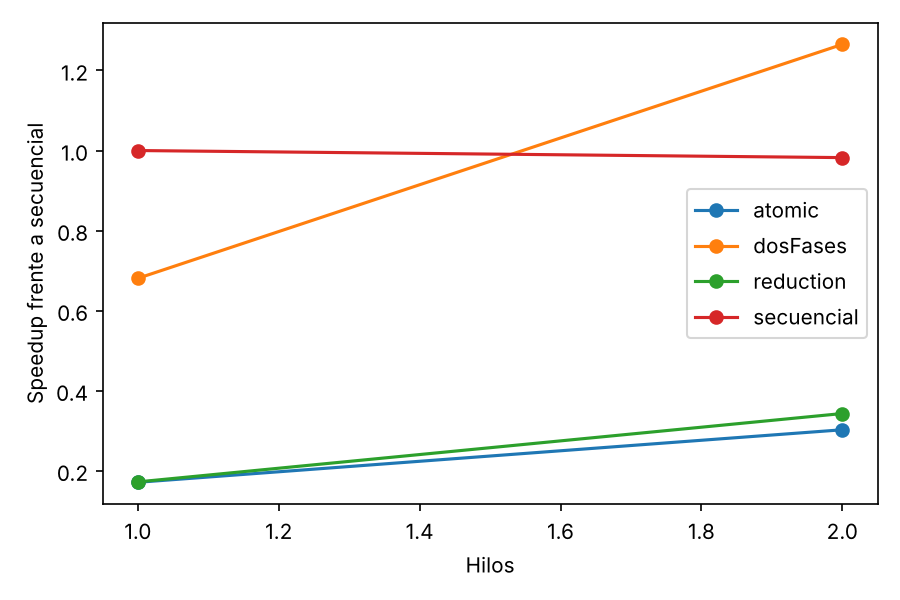
\includegraphics[width=0.62\linewidth]{figuras/speedup.png}
\caption{Speedup orientativo con 1 y 2 hilos (nube de 2 vCPU, $N=10^3$, $M=10^5$). No usar en la memoria.}
\label{fig:speedup}
\end{figure}

\alt Gnuplot, o pgfplots dentro de LaTeX (mejor integración tipográfica, más lento de iterar).

\section{Herramientas y entorno}\label{tema:herr}
\soporte{F0, F12 y F15}

\concepto{10.1 Git e identidad de autor}
\que Control de versiones. Cada commit guarda autor y \emph{committer}.

\porque Quieres que solo figures tú en el repositorio, y el enunciado valora mostrar la evolución incremental del código.

\como Configura una vez \texttt{git config user.name "Antonio Millán Rodríguez"} y \texttt{git config user.email "antoniomillanr45@gmail.com"}. Un commit por fase, con un mensaje que nombre la fase, y una etiqueta por punto de control (\texttt{git tag pc1}). Verifica la autoría con:
\begin{lstlisting}[language=bash]
git log --format='%an <%ae> | %cn <%ce>'
git log --format=%B | grep -iE "co-authored|claude"
\end{lstlisting}
El segundo comando no debe devolver nada. La rama \texttt{claude/fervent-bell-1ekfj8} tiene un commit con autor \emph{Claude}: si la fusionas, rehaz ese commit con tu identidad (\texttt{git cherry-pick} y \texttt{git commit --amend --reset-author}) en lugar de fusionarlo tal cual, y borra la rama remota.

\alt Ramas por fase con \emph{pull requests}: más ordenado, pero excesivo para un proyecto individual.

\concepto{10.2 Make}
\que Herramienta que recompila solo lo que ha cambiado según reglas de dependencias.

\porque Un \texttt{make all} y un \texttt{make test} son lo que el profesor ejecutará en el servidor.

\como Ver \fichero{docs/guia/codigo/Makefile} (probado): objetivos \texttt{all}, \texttt{grad}, \texttt{test} y \texttt{clean}, con \texttt{ARCH = -arch=sm\_89} como variable que se cambia en el servidor (\texttt{make grad ARCH=-arch=sm\_80}).

\alt CMake: detecta CUDA y OpenMP de forma portable, pero añade una capa de complejidad innecesaria para un proyecto de 10 ficheros.

\concepto{10.3 Contenedores: Docker y Apptainer}
\que Un contenedor empaqueta el sistema, las dependencias y el binario. Docker es el estándar general; Apptainer (antes Singularity; Kurtzer et al., 2017) es el habitual en servidores HPC porque no exige privilegios de \texttt{root}.

\porque El enunciado pide \emph{incluir la solución en un sistema de contenedores}, y sirve para fijar versiones (reproducibilidad).

\como Dockerfile orientativo (\fichero{docs/guia/codigo/Dockerfile}; no se ha podido construir en este entorno; etiqueta de imagen y compatibilidad de versiones con Ubuntu 22.04 \pv):
\begin{lstlisting}
FROM nvidia/cuda:12.4.1-devel-ubuntu22.04
RUN apt-get update && apt-get install -y --no-install-recommends make python3 python3-pip && rm -rf /var/lib/apt/lists/*
RUN pip3 install --no-cache-dir sympy==1.14.0 numpy==2.5.3 polars==2.1.0 matplotlib==3.11.2
WORKDIR /app
COPY . .
RUN make all grad
CMD ["make", "test"]
\end{lstlisting}
Ejecución con GPU: \texttt{docker run --gpus all imagen}; requiere NVIDIA Container Toolkit en el anfitrión. Con Apptainer: \texttt{apptainer build grad.sif docker-daemon://imagen:latest} y \texttt{apptainer run --nv grad.sif}.

\alt Podman (Docker sin demonio y sin \texttt{root}) o un entorno \texttt{conda}/\texttt{venv} más un \texttt{Makefile}: no es un contenedor y no cumple la tarea 6.

\begin{trampa}
La versión de CUDA de la imagen no puede ser más nueva de lo que admite el driver del servidor. Mira \texttt{nvidia-smi} (``CUDA Version'') antes de elegir la etiqueta.
\end{trampa}

\concepto{10.4 Librerías de Python}
\begin{center}\small
\begin{tabularx}{\linewidth}{@{}l l X@{}}
\toprule
Librería & Papel & Por qué sí o por qué no como base \\
\midrule
SymPy 1.14 & Validación (oráculo) & Exacta, pero lenta para $M>10^4$: solo casos pequeños \\
NumPy 2.5 & Generación & Generación vectorizada de enteros aleatorios con \texttt{default\_rng} \\
Polars 2.1 & Generación y análisis & Agregaciones rápidas de CSV de tiempos; Pandas también valdría \\
Matplotlib 3.11 & Análisis & Gráficas para la memoria \\
JAX o PyTorch & Comparación opcional & AD de referencia del estado del arte; no son base porque el enunciado pide C \\
\bottomrule
\end{tabularx}
\end{center}
Versiones probadas en esta guía; fíjalas en \fichero{requirements.txt}.

\concepto{10.5 Trabajo en el servidor de prácticas}
\que El entorno donde se harán las pruebas finales.

\porque Es obligatorio, y su hardware determina todos los resultados.

\como Copia con \texttt{git clone} (o \texttt{rsync}), compila allí con \texttt{ARCH} adaptado y lanza los benchmarks con \texttt{nohup ./reproduce.sh \&} o dentro de \texttt{tmux}. Si hay gestor de colas (Slurm), usa \texttt{sbatch} y pide los nodos en exclusiva \pv.

\alt Medir en el portátil sirve para desarrollar y como segundo entorno comparativo en la memoria, pero no sustituye al servidor.

\section{IA generativa, prompts y memoria}\label{tema:ia}
\soporte{F13 y F14 (apartados 2.1.4 y 2.1.5, 30\,\% en total)}

\concepto{11.1 Ingeniería de prompts}
\que Diseñar la petición a un modelo de lenguaje para obtener una respuesta útil: contexto, objetivo, restricciones, formato de salida y ejemplos.

\porque Se puntúa \emph{la calidad y el contexto} de los prompts y su refinamiento incremental.

\como Estructura de prompt que funciona para código:
\begin{enumerate}
\item Rol y contexto: asignatura, enunciado y estado actual del código (adjunto).
\item Tarea concreta y criterio de éxito verificable (``debe dar (8, 15, 8)'').
\item Restricciones: C11, OpenMP 4.5, sin comentarios, nomenclatura, sin dependencias.
\item Formato: solo el fichero, o un diff.
\item Iteración: pega el error de compilación o los tiempos medidos y pide un diagnóstico, no solo un arreglo.
\end{enumerate}
Ejemplo de refinamiento: ``paraleliza el gradiente con OpenMP'' $\rightarrow$ ``paraleliza \texttt{gradSec} sobre CSR con OpenMP evitando atómicos; propone dos variantes y explica su coste en memoria'' $\rightarrow$ ``la variante \emph{reduction} es 3 veces más lenta que el secuencial con 2 hilos; aquí están los tiempos; ¿por qué?''.

\alt Usar la IA solo para depurar o documentar (más seguro, menos material para el apartado). Lo valorado es mostrar el proceso completo, incluidas las respuestas erróneas y cómo las detectaste.

\concepto{11.2 Registro de interacciones}
\que Un diario en \fichero{docs/prompts.md}.

\porque Reconstruirlo al final es costoso y poco creíble. El enunciado pide, para cada IA: ámbito de uso, lista de prompts, soluciones obtenidas y valoración final.

\como Plantilla por entrada:
\begin{lstlisting}
## Fecha  IA y modelo  Fase
Prompt: ...
Respuesta resumida: ...
Fragmento clave: ...
Problema detectado y cómo: ...
Commit resultante: ...
\end{lstlisting}
Incluye esta guía como una interacción (ámbito: planificación y estudio).

\alt Exportar las conversaciones completas como anexo: útil como respaldo, pero el cuerpo de la memoria debe ser un análisis, no un volcado.

\concepto{11.3 Memoria con el esquema oficial}
\que El documento de entrega: Abstract, Introducción, El problema, Paralelización (secuencial, multinúcleo, GPU, extensiones), Resultados (entorno, resultados), Conclusiones y Bibliografía.

\porque Vale un 15\,\% y es lo que se lee antes de la entrevista.

\como Cada tema de esta guía alimenta una sección: 1 y 2 van a ``El problema''; 3, 5, 6, 7 y 8, a ``Paralelización''; 4 y 9, a ``Resultados''; 12, a ``Introducción''. Escribe cada sección al cerrar su fase, no al final. Cita solo referencias que hayas consultado.

\alt LaTeX (recomendado: fórmulas y bibliografía) o Markdown con Pandoc (más rápido, menos control).

\section{Estado del arte}\label{tema:arte}
\soporte{F14 (introducción) y contexto de todas}

\concepto{12.1 Diferenciación automática}
\que La técnica estándar para gradientes en aprendizaje automático y optimización (Baydin et al., 2018; Griewank y Walther, 2008). El modo inverso calcula el gradiente completo con un coste acotado por un pequeño múltiplo constante del coste de evaluar $f$ (principio del gradiente barato).

\porque Sitúa el proyecto: nuestro algoritmo prefijo-sufijo es un modo inverso especializado para productos, sin cinta (\emph{tape}) ni grafo, gracias a conocer la estructura polinómica.

\como Herramientas: PyTorch (\texttt{autograd}; Paszke et al., 2019), JAX (\texttt{grad}, \texttt{jit}, \texttt{vmap}; Bradbury et al., 2018), Enzyme (AD a nivel de LLVM, incluso de kernels CUDA; Moses y Churavy, 2020) y CasADi. Un experimento opcional valioso: comparar tu CUDA con \texttt{jax.grad} sobre el mismo polinomio en la misma GPU.

\alt --- (es el contexto, no una opción de implementación).

\concepto{12.2 Evaluación de polinomios y sus derivadas en GPU}
\que Existe trabajo específico sobre evaluar y diferenciar sistemas polinómicos en GPU para métodos de homotopía, por ejemplo Verschelde y Yoffe (2012) \pv. Usan, entre otras ideas, productos tipo Speelpenning para los monomios.

\porque Confirma que el planteamiento (monomio por hilo y productos prefijo y sufijo) es el adecuado y da una referencia seria para la introducción.

\como Lee el resumen y la sección de algoritmo antes de citarlo. Si no puedes acceder, no lo cites.

\alt SpMV en GPU (Bell y Garland, 2009) es el problema hermano: mismo patrón disperso, mismas técnicas (CSR, ELL, \emph{sliced} ELL). Sus conclusiones sobre formatos son directamente aplicables.

\concepto{12.3 En qué se diferencia este proyecto}
\begin{itemize}
\item Derivación exacta especializada en polinomios dispersos, sin grafo de AD: menos memoria y sin dependencias.
\item Comparación sistemática de estrategias de acumulación (\emph{reduction}, \emph{atomic}, dos fases) en CPU y GPU sobre el mismo problema.
\item Extensión al Jacobiano con un CSR global y estudio de anidado.
\item Documentación del uso de IA generativa como parte del método.
\end{itemize}
No es más rápido que una biblioteca de AD en general: es más rápido \emph{en este caso particular}, y eso es lo que hay que demostrar con medidas.
\clearpage

\section{Tabla de decisiones}\label{sec:decisiones}

{\footnotesize
\begin{xltabular}{\linewidth}{@{}>{\bfseries}p{0.6cm} >{\raggedright\arraybackslash}p{2.4cm} >{\raggedright\arraybackslash}p{3.0cm} >{\raggedright\arraybackslash}p{2.4cm} >{\raggedright\arraybackslash}X >{\raggedright\arraybackslash}p{0.8cm}@{}}
\toprule
Id & Decisión & Opciones & Recomendación & Motivo y qué medir para decidir & Fase \\
\midrule
\endfirsthead
\toprule
Id & Decisión & Opciones & Recomendación & Motivo y qué medir para decidir & Fase \\
\midrule
\endhead
\bottomrule
\endfoot
D1 & Lenguaje de las versiones paralelas & C, C++ & C (tomada) & Integración directa con OpenMP y CUDA; CUDA se compila como C++ con estilo C & F0 \\
D2 & Nombres de ficheros & \fichero{.cpp} actuales, \fichero{.c}/\fichero{.cu} & \fichero{.c} y \fichero{.cu} en \fichero{src/} & \texttt{nvcc} necesita \fichero{.cu}; coherencia con D1 & F0 \\
D3 & Sistema de compilación & Make, CMake & Make & Pocos ficheros; el profesor solo ejecuta \texttt{make} & F0 \\
D4 & Formato de validación & Texto del enunciado, CSV, binario & Texto con la regla letra+dígitos & Notación del enunciado y legible; base del oráculo & F1 \\
D5 & Formato de benchmark & Texto, CSV, binario & Binario si el parseo pesa & Medir el tiempo de parseo frente al de cálculo en el caso M: si el parseo supera el 10\,\% del total, binario & F1 \\
D6 & Rangos del generador & Los actuales ($e\le100$, $k\le100$), seguros & $c\le9$, $e\le5$, $k\le16$, $x\in[0.5,1.5]$ & Evita \texttt{inf}; comprobar que $\max|g_j|<10^{300}$ & F1 \\
D7 & Representación & Densa, COO, CSR, ELL & CSR (cambia la decisión densa del 18-oct) & Memoria $O(F)$; medir la densidad $F/(MN)$ de tus casos & F3 \\
D8 & Algoritmo por monomio & Ingenuo, división, prefijo-sufijo & Prefijo-sufijo & $O(k)$ sin divisiones; medida: el ingenuo es 3 veces más lento & F4 \\
D9 & Potencias & \texttt{pow}, bucle, cuadrados, tabla & Cuadrados; tabla en F9 si se mide mejora & Medir tiempo por factor con cada una en el caso M & F4, F9 \\
D10 & Precisión & \texttt{double}, \texttt{float}, mixta & \texttt{double}; \texttt{float} como experimento & Corrección exigida; medir tiempo y error (E10) & F4, F9 \\
D11 & Tolerancia & Absoluta, relativa, mixta & $\le10^{-12}\max(1,|g|)$ & Coeficientes positivos y $x\in[0.5,1.5]$; relajar con justificación si hay cancelación & F6 \\
D12 & Acumulación en OpenMP & \texttt{critical}, \texttt{atomic}, \texttt{reduction}, privatizada, dos fases & Dos fases como principal; las demás como comparación & Determinista y sin conflictos; medir las cinco frente a $N$ (E3, E8) & F7 \\
D13 & \texttt{schedule} & static, dynamic, guided, por factores & Decidir con datos; partir de dynamic,256 & Barrido E5; mirar la varianza entre hilos P y E & F7 \\
D14 & Anidado & Anidado real, \texttt{collapse}, \texttt{taskloop} & Estudiar las tres & El enunciado pide el estudio; medir E6 & F7 \\
D15 & Mapeo CUDA & Hilo por monomio, por factor, warp por monomio, dos fases & Hilo por monomio con atómicos (base) y dos fases (optimizada) & Corrección primero; comparar en E7 y E8 & F8, F9 \\
D16 & Tamaño de bloque & 32 a 1024 & Elegir por barrido & Medir E7 y contrastar con la ocupación teórica & F8 \\
D17 & Memoria para \texttt{vX} & Global con \texttt{\_\_ldg}, compartida, constante & \texttt{\_\_ldg}; compartida si $N\le6144$ y mejora & Constante descartada por los accesos divergentes; medir con \texttt{ncu} & F9 \\
D18 & Layout en GPU & CSR, ELL transpuesto, sliced ELL ordenado & CSR; probar sliced ELL & Medir el ancho de banda efectivo y la eficiencia de warp & F9 \\
D19 & Estructura del sistema & $K$ \texttt{Poli} separados, CSR global & CSR global con \texttt{vIdEc} & Un solo bucle o kernel equilibrado & F10 \\
D20 & Almacenamiento de $J$ & Denso, disperso & Denso hasta unos 100 MB & $8KN$ bytes; disperso por encima & F10 \\
D21 & Contenedor & Docker, Apptainer, Podman & Según el servidor & Preguntar si hay Docker con NVIDIA Container Toolkit o Apptainer y si hay \texttt{root} & F12 \\
D22 & Paralelismo en Rust & Ninguno, rayon & Ninguno & Fuera del enunciado; solo secuencial & F5 \\
D23 & Qué tiempos se reportan & Solo cálculo, total & Ambos, separados & El enunciado pide el desglose; Amdahl exige conocer la parte secuencial & F11 \\
\end{xltabular}
}

\section{Experimentos, riesgos y calendario}\label{sec:experimentos}

\subsection{Experimentos planificados}

Casos de tamaño (definidos en el concepto 2.3): S ($N=10^3$, $M=10^4$), M ($N=10^4$, $M=10^6$) y L ($N=10^5$, $M=10^7$), todos con $k\in[1,16]$, $e\in[1,5]$, $c\in[1,9]$, $x\in[0.5,1.5]$, semilla de función 0 y semilla de punto 1. Hilos: $\{1,2,4,6,8,12\}$ en el portátil y potencias de 2 hasta el número de núcleos en el servidor. $R=10$ repeticiones y mediana.

{\footnotesize
\begin{xltabular}{\linewidth}{@{}>{\bfseries}p{0.6cm} >{\raggedright\arraybackslash}p{3.0cm} >{\raggedright\arraybackslash}p{4.6cm} >{\raggedright\arraybackslash}X@{}}
\toprule
Id & Objetivo & Configuración & Resultado esperado \\
\midrule
\endfirsthead
\toprule
Id & Objetivo & Configuración & Resultado esperado \\
\midrule
\endhead
\bottomrule
\endfoot
E1 & Corrección & Ejemplo del enunciado; sistema del enunciado; oráculo ($N=50$, $M=200$, semilla 7; $N=300$, $M=2000$, semilla 11); casos límite del concepto 9.1 & $(8,15,8)$; filas $(6,3,3)$, $(4,27,54)$, $(9,24,25)$; error 0 frente al oráculo (ya obtenido con el prototipo) \\
E2 & Coste secuencial & C, C++ y Rust en S, M y L & Tiempo lineal en $F$ (unos 16 ns por factor en la nube); diferencias entre lenguajes por debajo del 20\,\% \pv \\
E3 & Escalado fuerte OpenMP & Caso M, cinco variantes de D12, todos los hilos & Dos fases con mejor eficiencia; \emph{reduction} empeora al crecer los hilos por la fusión $O(pN)$; techo por ancho de banda \\
E4 & Escalado débil OpenMP & $M=10^5\cdot p$, $N=10^4$ & Tiempo casi constante hasta saturar el ancho de banda \\
E5 & Planificación & Caso M, 8 hilos, static, dynamic y guided con trozos $\{16,64,256,1024,4096\}$ & dynamic o guided por encima de static en el portátil (núcleos P y E); trozo pequeño penalizado \\
E6 & Anidado & $P\in\{1,16,256\}$ puntos, caso S, todas las combinaciones $h_{\text{ext}}\times h_{\text{int}}$ & Con $P=256$ gana el externo o \texttt{collapse}; con $P=1$ solo sirve el interno \\
E7 & CUDA: bloque y desglose & Casos S, M y L; bloques de 32 a 1024; \texttt{kMonoAtom} y dos fases & H2D mayor que el kernel en una evaluación; 32 hilos por bloque peor; meseta entre 128 y 512 \\
E8 & Contención de atómicos & $F=8.5\cdot10^6$ fijo y $N\in\{10,10^3,10^5\}$; CPU y GPU & Atómicos muy lentos con $N=10$; dos fases insensible a $N$ \\
E9 & Jacobiano & $K\in\{10,100,1000\}$, $N=10^3$, $M=10^3$ por ecuación & CSR global equilibrado; denso hasta $K=1000$ (8 MB) \\
E10 & \texttt{float} frente a \texttt{double} & Caso M en GPU & \texttt{float} más rápido en GeForce; error relativo del orden de $10^{-6}$ \\
E11 & Lotes de puntos en GPU & Caso M con 1, 10 y 100 puntos y estructura residente & El coste de H2D se amortiza; speedup frente al secuencial creciente con los puntos \\
\end{xltabular}
}

\subsection{Riesgos}

{\footnotesize
\begin{xltabular}{\linewidth}{@{}>{\raggedright\arraybackslash}p{4.2cm} >{\raggedright\arraybackslash}p{1.6cm} >{\raggedright\arraybackslash}X@{}}
\toprule
Riesgo & Impacto & Mitigación \\
\midrule
\endhead
\bottomrule
\endfoot
CUDA no coincide con el secuencial (eliminatorio) & Muy alto & Validar contra el oráculo en cada commit; casos límite; comprobar errores CUDA; comparar con tolerancia, no con \texttt{==} \\
Servidor sin GPU disponible, ocupado o con otro modelo & Alto & Medir pronto (PC3); tener resultados del portátil como respaldo y declararlo; \texttt{ARCH} parametrizado \\
Driver del servidor incompatible con la versión de CUDA o del contenedor & Medio & \texttt{nvidia-smi} y \texttt{nvcc --version} la primera semana; elegir la imagen según el driver \\
Docker no permitido en el servidor & Medio & Apptainer con \texttt{--nv}; si nada funciona, documentarlo y entregar el Dockerfile probado en el portátil \\
Desbordamientos o \texttt{inf} en casos grandes & Medio & Rangos de D6; comprobar \texttt{isfinite} en los tests \\
El parseo domina el tiempo y oculta el speedup & Medio & Medir por separado; formato binario (D5) \\
Medidas ruidosas por compartir el servidor & Medio & Mediana de 10, afinidad, horas valle, anotar la carga \\
Retraso en la parte de IA y memoria (30\,\%) & Alto & Registrar prompts desde ya; escribir cada sección al cerrar su fase \\
Fecha de entrega desconocida & Alto & Confirmarla esta semana en el aula virtual; ajustar el calendario \\
Ambigüedades del enunciado (pesos, formato, contenedores) & Medio & Preguntar al profesor por escrito y citar la respuesta en la memoria \\
Pérdida de trabajo & Medio & Push diario; etiquetas por punto de control \\
\end{xltabular}
}

\subsection{Calendario con puntos de control}

\supuesto{entrega opcional de OpenMP hacia el 7-dic-2026 y entrega final hacia el 25-ene-2027. Ajusta las fechas cuando confirmes las reales.}

{\footnotesize
\begin{xltabular}{\linewidth}{@{}>{\raggedright\arraybackslash}p{2.3cm} >{\raggedright\arraybackslash}p{2.6cm} >{\raggedright\arraybackslash}X >{\raggedright\arraybackslash}p{4.0cm}@{}}
\toprule
Semana & Fases & Punto de control: qué debe estar listo & Si no lo está \\
\midrule
\endhead
\bottomrule
\endfoot
2--8 nov & F0, F1 & Repo reorganizado, generadores con semilla, entorno del servidor guardado & Usar el \fichero{generador.py} existente con los rangos de D6 \\
9--15 nov & F2, F3, F4 & \textbf{PC1}: secuencial en C validado con el ejemplo y el oráculo & Usar los prototipos de esta guía tal cual y seguir \\
16--22 nov & F5, F6 & C++ y Rust; \texttt{make test} en verde & Posponer Rust: no puntúa en el enunciado \\
23--29 nov & F7 & Cinco variantes OpenMP correctas & Quedarse con \emph{reduction} y dos fases \\
30 nov--6 dic & F7, F11 (CPU) & \textbf{PC2}: escalabilidad, schedule y anidado medidos en el servidor; entrega opcional & Entregar con lo medido; el anidado puede ir después \\
7--13 dic & F8 & \textbf{PC3}: CUDA base correcto con desglose de tiempos en el servidor & Prioridad máxima: es eliminatorio. Pedir ayuda en tutoría \\
14--20 dic & F10, F9 & Jacobiano en secuencial, OpenMP y CUDA; primera optimización CUDA & F9 es opcional: saltarla antes que F10 \\
21 dic--10 ene & F11, F12 & \textbf{PC4}: todos los benchmarks en CSV y figuras; contenedor funcionando & Reducir la rejilla de experimentos a S y M \\
11--17 ene & F13, F14 & \textbf{PC5}: memoria completa en borrador y registro de IA cerrado & Recortar texto, no resultados \\
18--24 ene & F15 & \texttt{reproduce.sh} regenera todo; revisión final; ensayo de la entrevista & Entregar lo que hay: el contenido mínimo ya existe desde PC4 \\
\end{xltabular}
}

\section{Validación y reproducibilidad}\label{sec:validacion}

\textbf{Tests.} \texttt{make test} ejecuta: el ejemplo (\texttt{grad = (8, 15, 8)}), el sistema (fila \texttt{(9, 24, 25)}), los casos límite del concepto 9.1 y dos casos aleatorios contra el oráculo. Cada versión paralela se compara después con el secuencial en el caso M. El prototipo ya incluye los dos primeros en el \fichero{Makefile}.

\textbf{Tolerancias.}
\begin{center}\small
\begin{tabularx}{\linewidth}{@{}>{\raggedright\arraybackslash}p{5.2cm} l >{\raggedright\arraybackslash}X@{}}
\toprule
Comparación & Tolerancia & Motivo \\
\midrule
Secuencial frente a oráculo (puntos enteros) & $10^{-12}\max(1,|g|)$ & Error obtenido: 0 \\
Paralelo \texttt{double} frente a secuencial & $10^{-12}\max(1,|g|)$ & Solo cambia el orden de las sumas (obtenido $\le5.4\cdot10^{-15}$) \\
GPU \texttt{float} frente a secuencial & $10^{-4}\max(1,|g|)$ & $u_{\text{float}}\approx6\cdot10^{-8}$ por unos $10^3$ términos \\
\bottomrule
\end{tabularx}
\end{center}

\textbf{Semillas.} Función: 0; punto: 1; casos de oráculo: 7 y 11. Se escriben en la cabecera de cada fichero generado y en cada fila del CSV de tiempos.

\textbf{Versiones fijadas.} Las de la tabla \ref{tab:versiones}, en \fichero{requirements.txt} y en el Dockerfile. \fichero{reproduce.sh} guarda las del servidor en \fichero{resultados/entorno.txt}.

\begin{table}[h]
\centering\small
\begin{tabular}{@{}lll@{}}
\toprule
Herramienta & Versión probada en la guía & Servidor \\
\midrule
gcc & 13.3.0 (OpenMP 4.5 o superior) & Por medir \\
nvcc & 12.0.140 (solo compilación) & Por medir \\
rustc & 1.97.0 & Por medir \\
Python & 3.13 & Por medir \\
SymPy, NumPy, Polars, Matplotlib & 1.14.0, 2.5.3, 2.1.0, 3.11.2 & Fijar en \fichero{requirements.txt} \\
\bottomrule
\end{tabular}
\caption{Versiones.}\label{tab:versiones}
\end{table}

\textbf{Metodología de medida.} La del concepto 9.2: calentamiento, $R=10$, mediana y desviación, afinidad, tiempos separados por etapa y verificación de cada ejecución medida.

\textbf{Script único.} \fichero{reproduce.sh} (probado en la parte de CPU): guarda el entorno, compila, pasa los tests y el oráculo, ejecuta los benchmarks, genera las gráficas y, si hay GPU, barre los tamaños de bloque.
\begin{lstlisting}[language=bash]
make all
make test
for caso in "50 200 7" "300 2000 11"; do
  python3 oraculo.py $caso
  gcc -O2 -o compara compara.c poli.c -lm
  ./compara
done
./bench.sh 1000 100000 5 resultados/tiempos.csv
python3 graficas.py resultados/tiempos.csv
if command -v nvidia-smi > /dev/null; then
  make grad
  for b in 32 64 128 256 512 1024; do ./grad 10000 1000000 "$b"; done > resultados/cuda.txt
fi
\end{lstlisting}
Al llevarlo al repositorio final, amplía \fichero{bench.sh} a la rejilla de la sección \ref{sec:experimentos}.

\section{Orientación a la entrega académica}\label{sec:entrega}

El objetivo externo es la entrega de la práctica y, en tu caso, una nota de 9 o más para optar a matrícula de honor. Cómo orientar el trabajo:
\begin{itemize}
\item \textbf{Asegura lo eliminatorio primero}: CUDA correcto (PC3) vale más que cualquier optimización.
\item \textbf{Rúbrica implícita}: cada requisito del enunciado debe tener una tabla o gráfica con nombre propio en la memoria: \texttt{omp\_get\_wtime}, escalabilidad, anidado, desglose CUDA, tamaños de bloque, Jacobiano, contenedor, prompts.
\item \textbf{Análisis crítico}: para cada gráfica, una explicación causal (Amdahl, ancho de banda, contención, desequilibrio) apoyada en una medida adicional (\texttt{perf}, \texttt{ncu}, Karp-Flatt). Es lo que separa un 7 de un 9.
\item \textbf{Parte opcional de CUDA}: con dos optimizaciones bien medidas (dos fases y ordenación por longitud, por ejemplo) y una descartada con datos basta para destacar.
\item \textbf{IA (15\,\%)}: muestra la evolución, los errores de la IA que detectaste (por ejemplo, un \texttt{reduction} ingenuo $O(k^2)$ o un \texttt{atomicAdd} con CAS obsoleto) y cómo afinaste los prompts.
\item \textbf{Entrevista}: debes poder explicar sin notas la fórmula del gradiente de un monomio, por qué CSR, por qué dos fases, qué mide cada evento CUDA y qué limita el speedup. Los temas 1, 2, 5 y 6 cubren esas preguntas.
\item \textbf{Bibliografía}: cita las referencias relevantes del enunciado (Chandra; Mattson et al.; Brownlee; OpenAI) y las de esta guía que hayas leído.
\end{itemize}

\section*{Referencias}\addcontentsline{toc}{section}{Referencias}
{\small
\begin{enumerate}[leftmargin=*,label={[\arabic*]}]
\item Amdahl, G. M. (1967). Validity of the single processor approach to achieving large scale computing capabilities. \emph{AFIPS Spring Joint Computer Conference}, 483--485.
\item Baydin, A. G., Pearlmutter, B. A., Radul, A. A. y Siskind, J. M. (2018). Automatic differentiation in machine learning: a survey. \emph{Journal of Machine Learning Research}, 18(153), 1--43.
\item Bell, N. y Garland, M. (2009). Implementing sparse matrix-vector multiplication on throughput-oriented processors. \emph{Proceedings of SC'09}.
\item Bradbury, J. et al. (2018). JAX: composable transformations of Python+NumPy programs. \url{https://github.com/jax-ml/jax}.
\item Brownlee, J. (2023). \emph{Prompt Engineering for Coders}. Machine Learning Mastery (citada en el enunciado).
\item Chandra, R. et al. (2001). \emph{Parallel Programming in OpenMP}. Morgan Kaufmann.
\item Goldberg, D. (1991). What every computer scientist should know about floating-point arithmetic. \emph{ACM Computing Surveys}, 23(1), 5--48.
\item Griewank, A. y Walther, A. (2008). \emph{Evaluating Derivatives: Principles and Techniques of Algorithmic Differentiation} (2.ª ed.). SIAM.
\item Gustafson, J. L. (1988). Reevaluating Amdahl's law. \emph{Communications of the ACM}, 31(5), 532--533.
\item Higham, N. J. (2002). \emph{Accuracy and Stability of Numerical Algorithms} (2.ª ed.). SIAM.
\item Hoefler, T. y Belli, R. (2015). Scientific benchmarking of parallel computing systems. \emph{Proceedings of SC'15}.
\item Hwu, W. W., Kirk, D. B. y El Hajj, I. (2022). \emph{Programming Massively Parallel Processors} (4.ª ed.). Morgan Kaufmann.
\item Knuth, D. E. (1997). \emph{The Art of Computer Programming, vol. 2: Seminumerical Algorithms} (3.ª ed.), sección 4.6.3. Addison-Wesley.
\item Kurtzer, G. M., Sochat, V. y Bauer, M. W. (2017). Singularity: scientific containers for mobility of compute. \emph{PLoS ONE}, 12(5), e0177459.
\item Mattson, T. G., Sanders, B. A. y Massingill, B. L. (2004). \emph{Patterns for Parallel Programming}. Addison-Wesley.
\item Meurer, A. et al. (2017). SymPy: symbolic computing in Python. \emph{PeerJ Computer Science}, 3, e103.
\item Moses, W. y Churavy, V. (2020). Instead of rewriting foreign code for machine learning, automatically synthesize fast gradients. \emph{NeurIPS 2020}.
\item NVIDIA. \emph{CUDA C++ Programming Guide} y \emph{CUDA C++ Best Practices Guide}. \url{https://docs.nvidia.com/cuda/} (versión según el toolkit del servidor).
\item OpenAI (2023). Best practices for prompt engineering with AI models (citada en el enunciado). \url{https://platform.openai.com/docs/guides/gpt-best-practices}.
\item OpenMP Architecture Review Board (2021). \emph{OpenMP Application Programming Interface, Version 5.2}. \url{https://www.openmp.org/specifications/}.
\item Paszke, A. et al. (2019). PyTorch: an imperative style, high-performance deep learning library. \emph{NeurIPS 2019}.
\item Saad, Y. (2003). \emph{Iterative Methods for Sparse Linear Systems} (2.ª ed.). SIAM.
\item Verschelde, J. y Yoffe, G. (2012). Evaluating polynomials in several variables and their derivatives on a GPU computing processor. \emph{IEEE IPDPS Workshops} \pv.
\item Williams, S., Waterman, A. y Patterson, D. (2009). Roofline: an insightful visual performance model for multicore architectures. \emph{Communications of the ACM}, 52(4), 65--76.
\end{enumerate}
}


\end{document}
